\documentclass[11pt,twoside,a4paper]{report}

% -----------------------------------------------------------------------------
% Imperial College London, Department of Computing: MSc Individual Project
% Complete dissertation draft.  Compile only from the repository root, because
% bibliography and generated-figure paths are rooted there.  Either run:
%   latexmk -pdf -interaction=nonstopmode -halt-on-error docs/DISSERTATION_FULL_REPORT.tex
% or use the manual sequence:
%   pdflatex docs/DISSERTATION_FULL_REPORT.tex
%   bibtex DISSERTATION_FULL_REPORT
%   pdflatex docs/DISSERTATION_FULL_REPORT.tex
%   pdflatex docs/DISSERTATION_FULL_REPORT.tex
% The Vancouver bibliography source is references.bib at the repository root.
% -----------------------------------------------------------------------------

\usepackage[margin=2.5cm,includeheadfoot]{geometry}
\usepackage[T1]{fontenc}
\usepackage[utf8]{inputenc}
\usepackage{lmodern}
\usepackage{microtype}
\usepackage{setspace}
\usepackage{amsmath,amssymb,mathtools}
\usepackage{booktabs,longtable,tabularx,array,multirow}
\usepackage{graphicx}
\usepackage{xcolor}
\usepackage{tikz}
\usetikzlibrary{arrows.meta,calc,fit,positioning,shapes.geometric}
\usepackage{enumitem}
\usepackage{fancyhdr}
\usepackage{caption}
\usepackage{subcaption}
\usepackage{float}
\usepackage{url}
\usepackage[numbers,sort&compress]{natbib}
\usepackage[hidelinks]{hyperref}
\usepackage[nameinlink,noabbrev]{cleveref}

\hypersetup{
  pdftitle={Measuring, Quantifying, and Mitigating Uncertainty in LLM-Based Argument-Strength Judgement},
  pdfauthor={Zhang Xiaoning},
  pdfsubject={MSc Individual Project},
  pdfkeywords={LLM-as-a-judge, argument quality, uncertainty quantification, automatic prompt optimisation}
}

\setstretch{1.08}
\setlength{\parindent}{1.5em}
\setlength{\parskip}{0.25em}
\setlength{\headheight}{14pt}
\setlist{nosep,leftmargin=*}
\captionsetup{font=small,labelfont=bf}
\setcitestyle{numbers,square,comma}

\pagestyle{fancy}
\fancyhf{}
\fancyhead[LE]{\nouppercase{\leftmark}}
\fancyhead[RO]{\nouppercase{\rightmark}}
\fancyfoot[C]{\thepage}

\newcommand{\reporttitle}{Measuring, Quantifying, and Mitigating Uncertainty in LLM-Based Argument-Strength Judgement}
\newcommand{\reportauthor}{Zhang Xiaoning}
\newcommand{\supervisorname}{Professor Francesca Toni}
\newcommand{\degreeprogramme}{MSc in Computing}
\newcommand{\universityname}{Imperial College London}
\newcommand{\departmentname}{Department of Computing}
\newcommand{\modelname}[1]{\textsc{#1}}
\newcommand{\winner}{\textsc{UQ--APO Winner}}
\newcommand{\CI}{95\% confidence interval}
\newcommand{\rawp}{\ensuremath{p_{\mathrm{raw}}}}
\newcommand{\holmp}{\ensuremath{p_{\mathrm{Holm}}}}
\newcommand{\R}{\mathbb{R}}
\newcommand{\ind}{\mathbb{I}}
\newcolumntype{Y}{>{\raggedright\arraybackslash}X}
\newcolumntype{C}{>{\centering\arraybackslash}X}
\definecolor{measureblue}{HTML}{1F77B4}
\definecolor{uqorange}{HTML}{E07A1F}
\definecolor{apogreen}{HTML}{2A8C66}
\definecolor{externalred}{HTML}{B44545}
\definecolor{softgrey}{HTML}{F2F4F7}

% Result figures are optional during text-only drafting.  A labelled placeholder
% is produced if a generated figure is not found at compile time.
\newcommand{\resultfigure}[2][]{%
  \IfFileExists{#2}{\includegraphics[#1]{#2}}{%
    \fbox{\parbox[c][4cm][c]{0.85\linewidth}{\centering Missing generated figure:\\
    \texttt{\detokenize{#2}}}}}}

\begin{document}

% =============================================================================
% FRONT MATTER
% =============================================================================

\begin{titlepage}
  \centering
  \vspace*{1.5cm}
  {\Large \universityname\par}
  \vspace{0.3cm}
  {\large \departmentname\par}
  \vfill
  {\huge\bfseries \reporttitle\par}
  \vspace{1.5cm}
  {\Large \reportauthor\par}
  \vspace{0.8cm}
  {\large Supervisor: \supervisorname\par}
  \vfill
  {\large MSc Individual Project --- Final Report\par}
  {\large \degreeprogramme\par}
  \vspace{0.5cm}
  {\large August 2026\par}
\end{titlepage}

\pagenumbering{roman}
\setcounter{page}{1}

\chapter*{Abstract}
\addcontentsline{toc}{chapter}{Abstract}

Large language models (LLMs) are increasingly used as automatic judges, yet a
single plausible score does not reveal whether a judgement is accurate, stable, or
robust to apparently innocuous choices in the evaluation protocol.  This project
studies LLM-based pointwise scoring of supporting and attacking arguments, with
ranking accuracy first evaluated against synthetically designed reference orders and
then against two independent human-annotated resources.  It develops a single
experimental narrative from measurement, through uncertainty quantification (UQ),
to uncertainty-aware mitigation.

Three baseline studies compare three open-weight judges, four controlled prompt
families, hard and soft decoding, and visible reasoning.  Overall pairwise accuracy
on the internal four-argument dataset is high, but errors concentrate sharply among
adjacent arguments.  No manually designed prompt produces a robust cross-model
accuracy improvement.  Hard decoding guarantees parseability and greatly reduces
generation cost, but can alter model-dependent score distributions.  Visible
reasoning makes Qwen more decisive and reduces ties, yet also increases disagreement
between stochastic repetitions.

The project then introduces a prospective UQ protocol in which five scoring runs
define uncertainty and five disjoint runs define future risk.  Repeated-score
variance predicts future numerical deviation, while inverse pairwise margin strongly
discriminates future ranking errors in the internal domain.  These signals guide an
embedding-assisted discrete automatic prompt optimisation algorithm.  The selected
readable prompt achieves competitive internal accuracy and significantly lower Qwen
flip rates than three of four manual baselines.  However, this stability advantage
does not transfer to Mistral or to two independent human-annotated argument-quality
datasets.  External experiments show partial transfer of risk ranking but severe
degradation of probability calibration.  Finally, a Bayesian adaptive policy saves
generations by allocating more samples to uncertain cases, whereas a strict
claim-level conformal rule is valid but abstains everywhere with the available
calibration sample.

The central finding is that LLM-judge reliability is multi-dimensional and
distribution-dependent.  Accuracy, repeated-run stability, calibration, protocol
sensitivity, and cost must be reported jointly; improving one dimension in-domain
does not establish transferable reliability.

\chapter*{Acknowledgements}
\addcontentsline{toc}{chapter}{Acknowledgements}

I would like to thank my supervisor, Professor Francesca Toni, for her guidance and
feedback throughout this project.  I am also grateful to the researchers who made
the argument-quality datasets and open-weight language models used in this work
available to the research community.

\tableofcontents
\clearpage
\listoffigures
\addcontentsline{toc}{chapter}{List of Figures}
\clearpage
\listoftables
\addcontentsline{toc}{chapter}{List of Tables}
\clearpage

\chapter*{Abbreviations and notation}
\addcontentsline{toc}{chapter}{Abbreviations and notation}
\begin{longtable}{@{}p{0.20\textwidth}p{0.73\textwidth}@{}}
\toprule
Symbol or term & Meaning \\
\midrule
APO & Automatic prompt optimisation. \\
ECE & Expected calibration error. \\
LLM & Large language model. \\
UQ & Uncertainty quantification. \\
WA & Weighted-average human argument-quality score in IBM-ArgQ-Rank-30k. \\
$c$ & A claim. \\
$a_{ci}$ & Argument $i$ associated with claim $c$. \\
$s_{cir}$ & Score assigned to $a_{ci}$ in stochastic run $r$. \\
$y_{cij}$ & Reference preference between arguments $i$ and $j$. \\
$\widehat y_{cij}$ & Model-induced preference between arguments $i$ and $j$. \\
\bottomrule
\end{longtable}

\clearpage
\pagenumbering{arabic}
\setcounter{page}{1}

% =============================================================================
\chapter{Introduction}
\label{chap:introduction}
% =============================================================================

\section{Motivation}

Evaluating the quality of natural-language arguments is important for deliberation,
claim verification, decision support, and the assessment of generated content.
Human evaluation remains the most defensible source of construct validity, but it is
slow and costly.  LLMs offer a scalable alternative: a judge model can read a claim
and an argument, assign a numerical score, and thereby induce a ranking over several
arguments.  The attraction of this approach is also its danger.  A fluent score is
easy to parse as a measurement even when it changes with the prompt, the decoding
rule, visible reasoning, the model family, or the random seed.

Existing LLM-as-a-judge work has established that strong models can align with human
preferences on some tasks, while also exhibiting position, verbosity, authority,
and task-dependent biases \cite{zheng2023judging,chen2024judgement,bavaresco2025llmjudges,shi2025positionbias}.
Argument-strength judgement presents an especially demanding case.  The distinction
between an obviously poor argument and a strong one may be easy, whereas the order
between two plausible adjacent arguments can depend on factuality, relevance,
logical cogency, rhetorical force, and the relation of the argument to the claim.
Consequently, high aggregate accuracy can conceal instability exactly where the
measurement is most scientifically interesting.

This dissertation treats an LLM judge as a stochastic measurement instrument rather
than a deterministic oracle.  The object of study is not merely whether one prompt
achieves the largest mean accuracy.  It is whether the instrument is accurate,
repeatable, calibrated, robust across protocols and domains, and sufficiently cheap
for practical use.

\section{Problem statement}

Let a pointwise judge assign an integer score in $\{0,\ldots,100\}$ to each argument
independently.  The scores induce pairwise preferences and a complete order.  The
same model can produce different scores under repeated stochastic generation, and
different protocols can alter both the score scale and the ranking.  The project
addresses three connected problems:

\begin{enumerate}
  \item \textbf{Measurement:} determine how model, prompt, decoding, and reasoning
  affect accuracy, stability, and cost.
  \item \textbf{Uncertainty:} determine whether dispersion observed in one set of
  scoring runs predicts errors and instability in disjoint future runs.
  \item \textbf{Mitigation:} use uncertainty to guide automatic prompt search and
  adaptive inference, then test whether the apparent gains generalise.
\end{enumerate}

The resulting research trajectory is therefore:
\begin{center}
\emph{measuring reliability $\rightarrow$ identifying uncertainty $\rightarrow$
automatically mitigating risk $\rightarrow$ testing transfer.}
\end{center}

\begin{figure}[htbp]
\centering
\resizebox{\textwidth}{!}{%
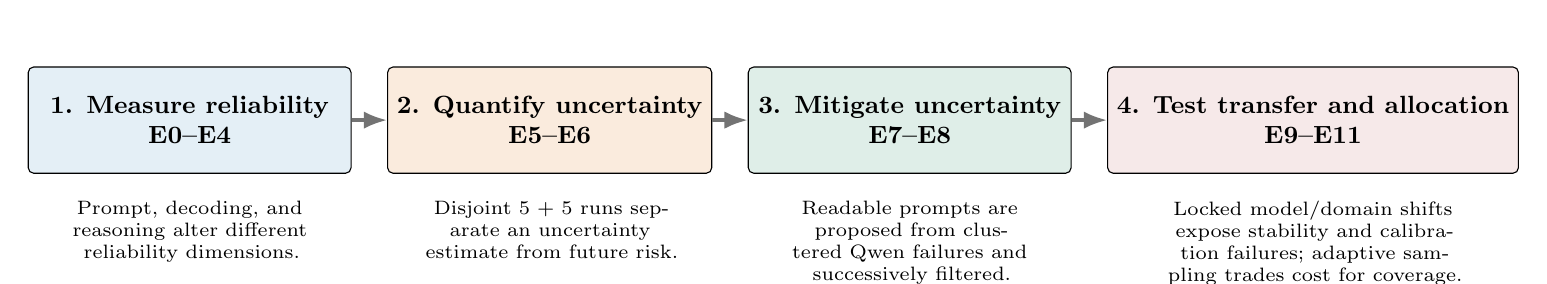
\begin{tikzpicture}[
  >=Latex,
  stage/.style={draw,rounded corners=2pt,minimum width=4.1cm,minimum height=1.35cm,
    align=center,font=\small\bfseries},
  finding/.style={align=center,text width=3.8cm,font=\scriptsize},
  link/.style={->,very thick,draw=black!55}
]
\node[stage,fill=measureblue!12] (measure) {1. Measure reliability\\E0--E4};
\node[stage,fill=uqorange!15,right=0.45cm of measure] (uq) {2. Quantify uncertainty\\E5--E6};
\node[stage,fill=apogreen!15,right=0.45cm of uq] (apo) {3. Mitigate uncertainty\\E7--E8};
\node[stage,fill=externalred!12,right=0.45cm of apo] (test) {4. Test transfer and allocation\\E9--E11};
\draw[link] (measure) -- (uq);
\draw[link] (uq) -- (apo);
\draw[link] (apo) -- (test);
\node[finding,below=0.22cm of measure] {Prompt, decoding, and reasoning alter different reliability dimensions.};
\node[finding,below=0.22cm of uq] {Disjoint $5+5$ runs separate an uncertainty estimate from future risk.};
\node[finding,below=0.22cm of apo] {Readable prompts are proposed from clustered Qwen failures and successively filtered.};
\node[finding,below=0.22cm of test] {Locked model/domain shifts expose stability and calibration failures; adaptive sampling trades cost for coverage.};
\end{tikzpicture}}
\caption{Overall research pipeline.  The design moves from diagnosing an LLM judge
as a stochastic measurement instrument to prospective UQ, automatic mitigation,
and deliberately adversarial tests of transfer.}
\label{fig:research-pipeline}
\end{figure}

\section{Research questions}
\label{sec:research-questions}

\begin{description}
  \item[RQ1:] How accurate and repeatable are open-weight LLM judges for
  argument-strength ranking, and do manually designed Role and Rubric prompts provide
  robust improvements over a Direct prompt?
  \item[RQ2:] Do hard output constraints and visible reasoning change the measured
  score, ranking, stability, or computational cost?
  \item[RQ3:] Which black-box repeated-sampling UQ signals predict errors and
  instability in disjoint future generations?
  \item[RQ4:] Can UQ-guided, embedding-assisted discrete prompt optimisation improve
  the accuracy--stability--cost profile of a target judge?
  \item[RQ5:] Do prompt and UQ gains transfer to another model and to independent,
  human-annotated argument-quality datasets?
  \item[RQ6:] Can Bayesian or conformal uncertainty policies reduce generation cost
  while retaining useful coverage and accuracy?
\end{description}

\section{Contributions}

The dissertation makes six empirical and methodological contributions.

\begin{enumerate}
  \item A controlled comparison of three open-weight judges and a $2\times2$ manual
  prompt design, evaluated with claim-grouped ranking and repeated-run metrics.
  \item Evidence that decoding and visible reasoning are parts of the measurement
  protocol: hard constraints may change model behaviour, while greater decisiveness
  need not imply greater epistemic certainty.
  \item A prospective $5+5$ UQ design that separates uncertainty estimation from
  future outcomes and evaluates discrimination, calibration, and selective risk.
  \item A reproducible UQ-aware APO loop that keeps prompts readable while using
  embeddings to diversify failures and remove semantically duplicate candidates.
  \item Locked internal, cross-model, and two-dataset external evaluations showing a
  distinction between in-domain improvement, risk-ranking transfer, and calibration
  transfer.
  \item An exploratory adaptive inference policy that translates UQ into a practical
  cost--coverage--risk trade-off.
\end{enumerate}

No claim is made to have introduced a new neural architecture, a new foundation
model, or a universal theory of uncertainty.  The contribution is an integrated and
carefully controlled reliability pipeline for a specific but consequential LLM-judge
task.

\section{Report structure}

\Cref{chap:related-work} reviews argument quality, LLM judges, prompting, and UQ.
\Cref{chap:methodology} defines the shared task, data, metrics, and statistical
principles.  \Cref{chap:baseline} establishes baseline reliability and protocol
effects.  \Cref{chap:uq} presents prospective UQ; \cref{chap:apo} presents the
automatic optimisation algorithm and internal evaluation.  \Cref{chap:external}
tests external generalisation, and \cref{chap:adaptive} converts uncertainty into an
adaptive inference policy.  \Cref{chap:evaluation} integrates the evidence and
limitations.  \Cref{chap:conclusion} concludes and identifies future work.

% =============================================================================
\chapter{Literature Review and Related Work}
\label{chap:related-work}
% =============================================================================

\section{Computational argument quality}

Argument quality is not a single surface property.  Wachsmuth et al. organise it
around logical, rhetorical, and dialectical dimensions, including cogency,
effectiveness, and reasonableness \cite{wachsmuth2017computational}.  This taxonomy
clarifies why a judge can disagree with a reference order even when both judgements
are superficially plausible: factual support, inferential strength, relevance, and
persuasiveness may conflict.

Large-scale data resources operationalise argument quality through pointwise or
pairwise human judgements.  Toledo et al. introduced datasets and supervised methods
for automatic argument-quality assessment \cite{toledo2019automatic}.
IBM-ArgQ-Rank-30k provides human quality scores for thousands of arguments across
topics and stances \cite{gretz2020largescale}.  Webis-ArgQuality-20 instead provides
efficient pairwise annotations along logical, rhetorical, and dialectical
dimensions \cite{gienapp2020efficient}.  The two resources are complementary in this
project: IBM supports broad versus near-tie ranking panels, whereas Webis supports a
direct human pairwise replication and dimension-specific sensitivity analyses.

\section{LLMs as judges}

LLM-as-a-judge evaluation became prominent through benchmarks such as MT-Bench and
Chatbot Arena, which showed useful agreement with human preferences while also
documenting position and style biases \cite{zheng2023judging}.  G-Eval demonstrated
that explicit evaluation criteria and structured reasoning can improve alignment for
natural-language generation evaluation \cite{liu2023geval}.  These findings motivate
the Rubric condition in this dissertation, but they do not guarantee that a rubric
will improve every model or construct.

More recent large-scale evidence cautions against treating LLM judges as generic
human substitutes.  Across 20 NLP tasks, Bavaresco et al. found substantial
model--dataset variability and argued for task-specific validation against human
judgements \cite{bavaresco2025llmjudges}.  Chen et al. identified judgement biases
under several controlled perturbations \cite{chen2024judgement}; Shi et al. showed
that position bias varies by judge, candidate, task, and quality gap
\cite{shi2025positionbias}.  Because the present system scores one argument at a
time, it avoids presentation-order bias between candidates during generation, but it
still requires ranking-level evaluation after scoring.

Reliability also includes stochastic consistency.  Xie et al. directly investigated
uncertainty in LLM evaluators and showed that it varies across model families and can
be used during evaluator training \cite{xie2025evaluatoruncertainty}.  The present
work is complementary: it uses black-box repeated scores, prospective held-out runs,
and readable-prompt optimisation rather than fine-tuning a judge.  Work on epistemic
markers further shows that merely verbalising uncertainty can itself bias an LLM
judge \cite{lee2025epistemicmarkers}.  This supports the decision to prioritise
behavioural dispersion over self-reported confidence.

\section{Prompt design and automatic optimisation}

The manual prompt study separates two common interventions: expert-role
conditioning and explicit evaluation criteria.  The factorial design is deliberately
simple.  Rather than attributing all prompt variation to an undifferentiated
``complexity'' effect, it estimates the Role and Rubric additions separately and in
combination.

Automatic prompt optimisation replaces manual iteration with a search procedure.
APE generates and evaluates natural-language instructions \cite{zhou2023ape};
ProTeGi uses textual critiques as gradient-like feedback with beam search
\cite{pryzant2023protegi}; and OPRO treats an LLM as an optimiser over natural-language
solutions \cite{yang2024opro}.  These methods primarily rank candidates by task
performance.  This dissertation instead records repeated-run variance, seed flips,
invalidity, calibration, completion tokens, and latency throughout the pipeline;
stability is active during screening, calibration becomes active in final validation,
and efficiency enters Pareto filtering rather than an active scalar token penalty in
the executed runs (\cref{chap:apo}).  Sentence-BERT embeddings
\cite{reimers2019sentencebert} assist clustering and deduplication, but the optimised
object remains a discrete, human-readable instruction.

\section{Reasoning, self-consistency, and constrained decoding}

Chain-of-thought prompting can improve multi-step reasoning \cite{wei2022chain}, and
self-consistency can improve final-answer accuracy by aggregating multiple reasoning
paths \cite{wang2023selfconsistency}.  Those results do not imply that a visible trace
will improve the reliability of scalar judgement.  In an evaluation task, reasoning
may make the judge more decisive while increasing between-run variance.  The
Reasoning Study therefore evaluates accuracy, ties, consistency, tokens, and latency
together.

Constrained decoding addresses a different problem.  Restricting generation to
legal score strings guarantees output validity but changes the model's output space.
Accordingly, this dissertation treats hard versus soft decoding as an experimental
factor rather than a neutral implementation detail.

\section{Uncertainty, calibration, and selective prediction}

Black-box LLM uncertainty can be estimated from repeated generations, output
agreement, entropy, and related dispersion measures.  Semantic entropy groups
semantically equivalent answers before computing uncertainty and has proved useful
for hallucination detection \cite{farquhar2024semanticentropy}.  The present task has
a fixed numerical output space, so score variance, option entropy, and pairwise
preference disagreement provide direct behavioural signals.  Xiong et al. show that
elicited confidence is not automatically reliable \cite{xiong2024uncertainty}, again
motivating behavioural rather than purely verbal confidence.

Discrimination and calibration are distinct.  A signal may rank risky cases well
without its predicted probabilities matching empirical frequencies.  Brier score and
expected calibration error are therefore reported alongside AUROC and AUPRC,
following the wider calibration literature \cite{guo2017calibration}.  Risk--coverage
analysis asks whether abstaining on the most uncertain cases reduces residual risk,
as in selective classification \cite{geifman2017selective}.

Conformal prediction offers finite-sample, distribution-free coverage under
exchangeability \cite{angelopoulos2023conformal}.  Its guarantees do not ensure useful
prediction-set size or low abstention.  This distinction is central to the adaptive
experiment, where a strict claim-level conformal construction is compared with a
practical Bayesian stopping rule.

\section{Research gap}

Prior work studies argument-quality prediction, LLM-judge bias, uncertainty,
prompt optimisation, and selective inference largely as separate questions.  The
unresolved issue is whether uncertainty can be measured prospectively, incorporated
into a readable-prompt search algorithm, and then shown to improve reliability under
locked internal and external evaluation.  This dissertation addresses that gap while
also testing a necessary boundary condition: whether internally optimised accuracy,
stability, and calibration survive model and dataset shift.

% =============================================================================
\chapter{Problem Formulation and General Methodology}
\label{chap:methodology}
% =============================================================================

\section{Task formulation}

For claim $c$, stance $r_c\in\{\text{support},\text{attack}\}$, and argument
$a_{ci}$, the judge produces
\begin{equation}
  s_{cir}=f_{\theta}(c,r_c,a_{ci};p,d,t,\omega_r)\in\{0,\ldots,100\},
  \label{eq:pointwise-score}
\end{equation}
where $p$ is the prompt, $d$ is the decoding protocol, $t$ is the reasoning mode,
and $\omega_r$ represents stochastic generation in run $r$.  Arguments are scored
independently.  For a pair whose reference order says $i$ is stronger than $j$,
\begin{equation}
  \widehat y_{cijr}=\operatorname{sign}(s_{cir}-s_{cjr})\in\{-1,0,1\}.
\end{equation}
Thus the generation task is pointwise, while its primary evaluation is pairwise.
This design avoids candidate-order effects during scoring and permits the same scores
to support pairwise, top-one, and full-order analyses.

\section{Datasets and data governance}
\label{sec:data-governance}

\subsection{Primary four-argument dataset}

The primary dataset contains 149 claims, of which 82 have supporting arguments and
67 have attacking arguments.  Each claim has four reference-ordered arguments,
yielding 596 pointwise scoring items and $149\times\binom{4}{2}=894$ unique argument
pairs per condition.  Reference ranks run from 1 (strongest) to 4 (weakest).

The immutable source artefact is
\path{datasets/5.15Dataset/true_false_uncertain_gen_gpt-5_ver_sonnet-4-5.jsonl}.
Its release filename records GPT-5 generation and Sonnet 4.5 verification as the
available provenance label.  Each JSONL record stores the claim, stance, four
arguments, and their designed rank order.  The repository snapshot does not contain
the upstream generation prompt, exact generator and verifier revisions, verification
rubric, rejection history, or annotator-level human labels.  Consequently, those
construction stages cannot be independently reconstructed from this release.  The
rank order is treated throughout as a \emph{synthetic benchmark reference}, not as a
human gold standard or an objective definition of argument strength.  E9 and E11
were added precisely to test conclusions against independent human annotations.

The dataset was used in the early baseline studies before the UQ/APO extension was
designed.  For the later algorithmic pipeline it was fingerprinted with SHA-256
\texttt{5710a2cf\ldots ad877b} and divided into claim-disjoint, stance-balanced
partitions (\cref{tab:internal-splits}).

\begin{table}[htbp]
\centering
\caption{Locked claim-disjoint UQ/APO partitions.}
\label{tab:internal-splits}
\begin{tabular}{lrrrr}
\toprule
Partition & Claims & Support & Attack & Permitted use \\
\midrule
APO training & 70 & 39 & 31 & Prompt search, promotion, full-training audit \\
Validation & 29 & 16 & 13 & UQ calibration and selection of one prompt \\
Internal test & 50 & 27 & 23 & One frozen evaluation; no rewriting or reselection \\
\bottomrule
\end{tabular}
\end{table}

The split was generated once with seed 20260802 and never regenerated.  It prevents
algorithmic leakage during APO, but it is not a pristine dissertation-level holdout:
aggregate results over all 149 claims had already been inspected in the Main Study.
This limitation is why two independent external datasets were added.

\subsection{IBM-ArgQ-Rank-30k external test}

E9 uses the official test partition of IBM-ArgQ-Rank-30k at fixed revision
\texttt{590726b3\ldots aa8a}.  Its 5,818 rows cover 15 topics.  Two topics selected by
a deterministic hash were used only for a format pilot and then completely excluded.
The formal test contains 13 unseen topics, two stances, and two four-argument panels
per topic--stance group: a \emph{broad} panel spanning human weighted-average quality
quantiles and a \emph{near-tie} panel drawn from the central quality band.  This
produces 52 claim records and 312 unique pairs.  Weighted-average quality is the
primary reference; MACE-P is secondary.  The formal file was fingerprinted before
generation and external results could not trigger prompt revision.

\subsection{Webis-ArgQuality-20 external test}

E11 uses Webis-ArgQuality-20 version 1.0.0 (DOI
\href{https://doi.org/10.5281/zenodo.3780049}{10.5281/zenodo.3780049}).  Arguments had
to be valid and pairs had to share both topic and stance.  Two hash-selected topics
were excluded after a format pilot.  The formal evaluation covers 18 topics, 36
topic--stance groups, 6,263 eligible dimension-labelled pairs, and 4,925 primary
majority-decisive pairs.  The primary reference is the majority direction across
logical, rhetorical, and dialectical human annotations; unanimous and
dimension-specific scopes are sensitivity analyses.

\subsection{Representation dataset}

The expanded/synonym file is derived from the primary claims.  It can test
representation sensitivity but cannot support a claim of external generalisation.
The corresponding E4 configuration exists, but no raw result was present at report
freeze.  E4 is therefore recorded as unexecuted in \cref{app:e4} and contributes no
empirical conclusion.

\section{Models and generation controls}

\begin{table}[htbp]
\centering
\caption{Open-weight models and frozen revisions.}
\label{tab:models}
\begin{tabularx}{\textwidth}{lYY}
\toprule
Short name & Hugging Face model & Revision \\
\midrule
Mistral-7B & \texttt{mistralai/Mistral-7B-Instruct-v0.3} & \texttt{c170c708\ldots bab71} \\
Qwen3-8B & \texttt{Qwen/Qwen3-8B} & \texttt{b968826d\ldots 91218} \\
GPT-OSS-20B & \texttt{openai/gpt-oss-20b} & \texttt{6cee5e81\ldots efebee} \\
\bottomrule
\end{tabularx}
\end{table}

The models were loaded in bfloat16 without additional quantisation.  Unless stated
otherwise, generation used sampling with temperature 0.7, top-$p$ 0.95, and
repetition penalty 1.0.  The original three seeds were 42, 1024, and 2026; promotion
added 31415 and 27182; ten-run UQ additionally used 16180, 57721, 65537, 99991, and
104729.  Exact model revisions, dataset fingerprints, and split manifests were
stored before the frozen evaluations.  Model architecture details are available in
the corresponding reports and model cards \cite{jiang2023mistral,yang2025qwen3,openai2025gptoss}.

No model weights were updated.  In APO, Qwen3-8B was the target scoring model and
GPT-OSS-20B was a separate optimiser that proposed instruction rewrites.  The
optimiser did not generate the final argument scores.

\section{Controlled prompt conditions}

The manual prompts form a $2\times2$ factorial design (\cref{tab:prompt-design}).
All conditions retain the same claim, stance, argument, 0--100 scale, and output
instruction.  They differ only in expert-role conditioning and explicit criteria.

\begin{table}[htbp]
\centering
\caption{Controlled manual prompt design.}
\label{tab:prompt-design}
\begin{tabularx}{\textwidth}{lccY}
\toprule
Prompt & Role & Rubric & Additional content \\
\midrule
Direct & No & No & Task, scale, and output format only \\
Role & Yes & No & Impartial expert analyst and consistent stance treatment \\
Rubric & No & Yes & Factuality, relevance, logical quality, effectiveness, and stance-specific relation \\
Role+Rubric & Yes & Yes & Both additions, allowing their interaction to be assessed \\
\bottomrule
\end{tabularx}
\end{table}

The exact instructions, including the frozen APO winner, appear in
\cref{app:prompts}.  Prompt labels describe experimental conditions rather than a
claim that one style is intrinsically superior.

\section{Decoding and score extraction}

\subsection{Hard decoding}

Hard decoding used a tokenizer-aware prefix trie over the 101 legal strings
\begin{equation}
  \mathcal V_{\mathrm{score}}=
  \{\texttt{Score: 0},\texttt{Score: 1},\ldots,\texttt{Score: 100}\}.
\end{equation}
At every generation step, tokens that could not continue a legal string were masked,
and EOS became legal only after a complete score.  Hard output was therefore exactly
parseable by construction, but the restriction changed the generated output space.
E1 and E2 retained a nominal 512-token ceiling, although the trie normally ended
after a few tokens.  Later UQ/APO and external runs used a 12-token maximum.

\subsection{Soft decoding}

Soft decoding imposed no token-level restriction.  After removing a completed
\texttt{</think>} block or selecting the final GPT-OSS channel, the parser accepted
an exact \texttt{Score: N} or exactly one labelled \texttt{Score}/\texttt{Final
Score} line using ``:'' or ``='', optionally followed by \texttt{/100}.  A labelled
score is a number explicitly introduced as the final score, rather than an arbitrary
number mentioned in an explanation.  Empty outputs, missing labels, multiple labelled
scores, and values outside 0--100 were invalid.  Invalid outputs were never imputed
as 50 or another fallback.

\subsection{Reasoning modes}

Qwen Think/No-Think used the native chat-template \texttt{enable\_thinking} option.
GPT-OSS used high- or low-reasoning control in the rendered prompt.  E3 used soft
decoding to permit a visible trace, with ceilings of 1,024 tokens for No-Think and
4,096 for Think.

\section{Outcome measures}

\subsection{Ranking accuracy}

For the set $\mathcal P_c$ of ordered reference pairs in claim $c$, pairwise accuracy
is
\begin{equation}
 \operatorname{Acc}_c=\frac{1}{|\mathcal P_c|}
 \sum_{(i,j)\in\mathcal P_c}
 \left[\ind(s_{ci}>s_{cj})+\tfrac12\ind(s_{ci}=s_{cj})\right].
 \label{eq:pair-accuracy}
\end{equation}
A tie receives half credit.  Exact directional accuracy, used in E11, instead treats
a predicted tie as wrong.  The Main Study's \emph{strict} accuracy is different
again: it requires the correct score difference to be at least 10 points.

Spearman's $\rho$ compares the reference and predicted ranks.  Top-one accuracy
requires the strongest argument to be selected.  Exact-order accuracy requires the
entire four-argument order to match; one local inversion makes the claim incorrect.
Rank distance $|i-j|\in\{1,2,3\}$ distinguishes adjacent from easy far-apart pairs.

\subsection{Repeated-run stability}

For each argument, score dispersion is summarised across seeds.  Pairwise seed
consistency is the modal preference proportion.  Flip rate records whether both
positive and negative directions appear across seeds:
\begin{equation}
 \operatorname{Flip}_{cij}=\ind\left(\exists r,r':
 \widehat y_{cijr}=1\land\widehat y_{cijr'}=-1\right).
\end{equation}
Tie rate is reported separately so that a system is not rewarded for avoiding flips
by returning ties everywhere.  Generated tokens, latency, invalidity, and exact-format
compliance capture efficiency and operational reliability.

Flip rate is an ``at least one reversal'' statistic: with more stochastic runs there
are more opportunities to observe both directions.  It is therefore compared only
between conditions with the same number of runs and the same scoring units.  Raw
flip rates from three-, five-, and ten-seed studies are not interpreted as directly
commensurate.  Where run counts or outcome granularity differ, preference entropy,
disagreement probability, and score variance provide more comparable descriptions.

\section{Statistical analysis}
\label{sec:statistics}

Claims were the independent units for the internal studies and topics for the
external studies.  Seed-level generations and the 252 UQ partitions are repeated
measurements, not independent samples.  Descriptive estimates are accompanied by
claim- or topic-grouped 95\% bootstrap intervals.  Paired contrasts use sign-flip or
permutation tests with the pairing unit preserved; E9 and E11 use 10,000 clustered
bootstrap resamples and 100,000 paired permutations.

When several contrasts answer one declared question, Holm's sequential procedure
controls the family-wise error rate \cite{holm1979simple}.  Tables report both
\rawp{} and \holmp{} so that multiplicity is transparent.  Statistical significance
uses $\alpha=.05$, but interpretation prioritises effect size and interval width.
Equivalence tests use two one-sided tests with bounds $\pm.02$ for pairwise accuracy
and $\pm.03$ for Spearman correlation.  A non-significant difference is not described
as proof of equivalence.

\section{Experiment map}

\begin{longtable}{@{}p{0.07\textwidth}p{0.22\textwidth}p{0.51\textwidth}p{0.12\textwidth}@{}}
\caption{Experiments in the report.}\label{tab:experiment-map}\\
\toprule
ID & Study & Primary purpose and design & Status \\
\midrule
\endfirsthead
\toprule
ID & Study & Primary purpose and design & Status \\
\midrule
\endhead
E0 & Output-length pilots & Validate reasoning-specific token ceilings and parsing diagnostics. & Complete \\
E1 & Decoding validation & 20 claims; three models; Hard versus Soft; Rubric; three seeds. & Complete \\
E2 & Main Study & 149 claims; three models; four prompts; Hard; No-Think; three seeds. & Complete \\
E3 & Reasoning Study & 50 claims; Qwen/GPT-OSS; four prompts; Think versus No-Think; three seeds. & Complete \\
E4 & Representation robustness & Derived synonym/expanded arguments; not an external test. & Not run \\
E5 & Locked development design & Claim-disjoint 70/29/50 split and fingerprints. & Complete \\
E6 & Prospective UQ & Ten runs, all 5+5 partitions, future-risk evaluation. & Complete \\
E7 & UQ-aware APO & Embedding-assisted readable-prompt search with GPT-OSS optimiser. & Complete \\
E8 & Frozen internal evaluation & Successive halving, validation selection, internal and Mistral tests. & Complete \\
E9 & IBM external test & Five prompts, 13 topics, broad/near-tie panels, ten seeds. & Complete \\
E10 & Adaptive inference & Bayesian stopping and strict split conformal abstention. & Complete; exploratory \\
E11 & Webis replication & Three prompts, 18 topics, human pairwise targets, ten seeds. & Complete \\
\bottomrule
\end{longtable}

% =============================================================================
\chapter{Baseline Reliability and Measurement-Protocol Effects}
\label{chap:baseline}
% =============================================================================

This chapter answers RQ1 and RQ2.  E0 validates the generation ceilings; E1 tests
decoding; E2 establishes the model--prompt baseline; and E3 tests visible reasoning.
The final section analyses rank distance, tie transitions, score-scale use, difficult
claims, cost, and equivalence.  These diagnostics motivate the prospective UQ work
in \cref{chap:uq}.

\section{E0: output-length pilots}

E0 sampled 10 claims with seed 2026, balanced between support and attack.  Four
manual prompts and soft decoding were used.  A capped pilot used a 512-token limit;
a natural-length pilot inspected Qwen3-8B and GPT-OSS-20B reasoning to the available
context window.  The purpose was operational rather than inferential: completion
length, truncation, labelled-score extraction, and exact-format compliance were used
to distinguish insufficient token budgets from judgement failure.  The resulting
mode-specific ceilings were 1,024 tokens for No-Think and 4,096 for Think in E3.

\section{E1: hard versus soft decoding}
\label{sec:e1}

\subsection{Design}

E1 sampled 20 claims (10 support and 10 attack) and evaluated GPT-OSS-20B,
Mistral-7B, and Qwen3-8B under the Rubric prompt.  Hard and soft decoding were paired
by claim, argument, and seed.  All conditions used No-Think and seeds 42, 1024, and
2026.  The study asks whether a syntactic output guarantee is measurement-neutral.

\subsection{Results}

\begin{table}[htbp]
\centering
\caption{E1 decoding results.  Accuracy gives half credit to ties; flip denotes a
positive and negative pairwise direction across the three seeds.}
\label{tab:e1-results}
\begin{tabular}{lrrrrrr}
\toprule
Model & Hard acc. & Soft acc. & Hard flip & Soft flip & Hard tok. & Soft tok. \\
\midrule
GPT-OSS-20B & .908 & .939 & .258 & .132 & 5.0 & 228.9 \\
Mistral-7B & .917 & .925 & .192 & .108 & 5.8 & 116.3 \\
Qwen3-8B & .908 & .908 & .092 & .092 & 6.0 & 6.0 \\
\bottomrule
\end{tabular}
\end{table}

Hard decoding achieved 100\% exact-format compliance by construction.  Mistral soft
decoding still achieved 100\% score extraction, but only 7.9\% of its outputs were
exactly the requested string; the labelled-score parser recovered the remainder.
Qwen's soft outputs were already short and score-like, so the two protocols were
nearly identical.  GPT-OSS and Mistral showed lower flip point estimates under soft
decoding, at the cost of two orders of magnitude more tokens.  The E1 sample is too
small to support a universal ordering of decoding methods.

\subsection{Interpretation}

Hard decoding is operationally valuable: it guarantees parseability and is much
cheaper.  It is nevertheless part of the measurement instrument rather than a
neutral post-processing step.  By suppressing every continuation outside
$\mathcal V_{\mathrm{score}}$, it can change the distribution from which the score
is produced.  E1 therefore supports the bounded conclusion that decoding
\emph{can} create model-dependent measurement effects; it does not show that soft
decoding is universally superior.

\section{E2: Main Study}
\label{sec:e2}

\subsection{Design}

E2 scored all four arguments for all 149 claims using three models, four prompt
conditions, and three seeds under Hard, No-Think generation.  The design contains
$149\times4\times3\times4\times3=21{,}456$ score generations.  The primary question
is whether Role, Rubric, or their combination provides a stable improvement over
Direct within and across models.

\subsection{Aggregate results}

\begin{table}[htbp]
\centering
\caption{E2 seed-averaged pairwise accuracy (95\% claim-bootstrap CI).}
\label{tab:e2-accuracy}
\begin{tabular}{lrrrr}
\toprule
Model & Direct & Role & Rubric & Role+Rubric \\
\midrule
GPT-OSS-20B & .910 [.890,.929] & .905 [.886,.923] & .919 [.901,.937] & .931 [.914,.948] \\
Mistral-7B & .908 [.888,.926] & .914 [.894,.933] & .918 [.899,.936] & .904 [.883,.924] \\
Qwen3-8B & .919 [.901,.937] & .925 [.909,.941] & .930 [.911,.947] & .931 [.914,.946] \\
\bottomrule
\end{tabular}
\end{table}

The range of point estimates is narrow (.904--.931), and no prompt has the same rank
ordering across all three models.  Role+Rubric is highest for GPT-OSS and narrowly
for Qwen, whereas Rubric is highest for Mistral.  Exact-order accuracy is much lower
(approximately .54--.57 overall): all six pairwise relations must be correct, so one
adjacent inversion invalidates the complete order.

No overall prompt contrast establishes a robust accuracy improvement after Holm
correction.  Stance-specific analyses identify conditional effects
(\cref{tab:e2-conditional}, moved to the statistical appendix) rather than a
universal prompt hierarchy.

These effects do not license a general statement that Rubric or Role+Rubric is
superior.  They occur in particular model--stance cells, and the same prompt addition
can be neutral or adverse elsewhere.

\subsection{Prompt capability conclusion}

Direct is the simplest condition and is not systematically worse.  Role does not
produce a stable standalone gain.  Rubric has the strongest theoretical basis and a
small positive tendency in several cells, with clear Mistral attack benefits.
Role+Rubric can help GPT-OSS attack arguments but has no stable extra interaction
benefit.  Manual prompt design therefore changes local behaviour, but the data do not
support a model-independent prompt recommendation.

\section{E3: Reasoning Study}
\label{sec:e3}

\subsection{Design}

E3 sampled 50 claims, balanced between support and attack.  Qwen3-8B and
GPT-OSS-20B were tested with all four prompts, soft decoding, both reasoning modes,
and three seeds.  In addition to ranking accuracy, the design measures ties,
score dispersion, seed consistency, flips, extraction, token use, and latency.  The
central distinction is between becoming more decisive and becoming more reliable.

\subsection{Aggregate effects}

\begin{table}[htbp]
\centering
\caption{E3 Think minus No-Think effects averaged over prompts.}
\label{tab:e3-effects}
\begin{tabularx}{\textwidth}{llrrrrr}
\toprule
Model & Metric & No-Think & Think & $\Delta$ & 95\% CI & \holmp{} \\
\midrule
GPT-OSS & Pairwise accuracy & .9571 & .9639 & .0068 & [-.0038,.0187] & .8903 \\
Qwen & Pairwise accuracy & .9167 & .9363 & .0196 & [.0008,.0392] & .1824 \\
Qwen & Tie rate & .0550 & .0208 & -.0342 & [-.0542,-.0167] & .0016 \\
Qwen & Score SD & 1.926 & 4.606 & 2.679 & [2.165,3.206] & .00030 \\
Qwen & Seed consistency & .9408 & .8864 & -.0544 & [-.0736,-.0364] & .00030 \\
Qwen & Flip rate & .0867 & .1592 & .0725 & [.0475,.1000] & .00030 \\
\bottomrule
\end{tabularx}
\end{table}

Qwen's accuracy increase does not survive multiplicity correction, whereas the
reduction in ties and deterioration in repeated-run stability do.  GPT-OSS shows no
comparable aggregate stability deterioration.  Thinking therefore has a strong
model interaction rather than a universal effect.

\subsection{What happened to Qwen's ties?}

On adjacent Qwen pairs, accuracy moves from .859 to .877 and tie rate from .085 to
.040, but seed flip increases from .135 to .275.  Of 66 pairs tied under No-Think,
49 move in the correct mean direction, 9 move in the wrong direction, and 8 remain
tied.  However, 39 of 66 disagree across Thinking seeds and 21 produce both correct
and wrong directions.  The transition counts show why a lower tie rate alone is not
evidence of resolved epistemic uncertainty.

\begin{figure}[htbp]
\centering
\resultfigure[width=.78\textwidth]{results/figures/extended_analysis/qwen_tie_transitions.pdf}
\caption{Qwen No-Think tie transitions under Thinking.  Mean transitions are often
correct, but seed-level disagreement remains high.}
\label{fig:qwen-ties}
\end{figure}

\subsection{Interpretation}

Visible reasoning often forces Qwen to choose a direction and many former ties move
correctly on average.  Yet the chosen direction is frequently irreproducible.  The
most defensible conclusion is therefore:
\begin{quote}
Thinking resolves numerical ties more reliably than it resolves epistemic
uncertainty.
\end{quote}
This mechanism result directly motivates repeated-sampling UQ.

\section{Cross-cutting diagnostic analyses}
\label{sec:cross-cutting}

\subsection{Rank distance}

\begin{table}[htbp]
\centering
\caption{Main Study pairwise accuracy by reference-rank distance, averaged over
prompts.}
\label{tab:rank-distance}
\begin{tabular}{lrrr}
\toprule
Rank distance & GPT-OSS & Mistral & Qwen \\
\midrule
1 (adjacent) & .857 & .860 & .874 \\
2 & .967 & .953 & .973 \\
3 (strongest versus weakest) & .992 & .982 & .989 \\
\bottomrule
\end{tabular}
\end{table}

Overall pairwise accuracy above .90 is partly driven by easy, far-apart pairs.
Adjacent arguments account for most error and most scientific ambiguity.  This also
explains why modest changes among boundary pairs can have little effect on the
overall mean but a large effect on exact-order accuracy.

\begin{figure}[htbp]
\centering
\resultfigure[width=.78\textwidth]{results/figures/extended_analysis/rank_distance_accuracy.pdf}
\caption{Pairwise accuracy by rank distance.  Error is strongly concentrated among
adjacent arguments.}
\label{fig:rank-distance}
\end{figure}

\subsection{Score-scale use}

All three models discretise the nominal 0--100 scale, typically in multiples of five.
Approximately 71\% of GPT-OSS Main Study scores, 79\% of Mistral scores, and 49\% of
Qwen scores are multiples of ten.  GPT-OSS's average within-claim range is about
47.9, compared with about 79 for Mistral and Qwen.  A fixed ten-point strict margin
therefore has different effective difficulty across models.  Rank-based outcomes
are used for the main comparison; scale-dependent strict accuracy is retained as a
sensitivity measure.

\subsection{Difficulty, cost, and equivalence}

Claim-level error concentration identified 20 difficult claims, 10 with high
cross-model disagreement, and 11 reference pairs meriting manual review.  Potential
causes include factual-knowledge dependence, ambiguity, close argument quality, and
conflicts between factuality and logical effectiveness.  These cases informed APO
failure acquisition but were not relabelled after observing model behaviour.

The accuracy--stability--cost Pareto analysis demonstrates that the highest accuracy
cell is not automatically the best operational judge.  For example, Qwen Rubric
No-Think achieves accuracy around .933 and consistency around .950 with approximately
5.9 tokens and .29 seconds, whereas Thinking can consume hundreds of tokens while
reducing stability.

Equivalence tests used practical bounds of $\pm.02$ pairwise accuracy and $\pm.03$
Spearman.  No core prompt contrast met the equivalence criterion after within-model
Holm correction.  The data therefore show neither robust universal improvement nor
sufficiently precise evidence that every complex prompt is practically equivalent
to Direct.

\section{Chapter conclusion}

The baseline studies establish four requirements for later experiments.  First,
reliability must include stability and cost, not only mean accuracy.  Secondly,
boundary pairs require separate analysis.  Thirdly, repeated generations expose
uncertainty hidden by one decisive answer.  Finally, prompt and protocol effects are
model-dependent.  These findings motivate a prospective UQ design rather than
further intuition-led prompt editing.

% =============================================================================
\chapter{Prospective Uncertainty Quantification}
\label{chap:uq}
% =============================================================================

\section{E5: locked development design}

Before automatic optimisation, the primary dataset was fingerprinted and divided
into the fixed 70/29/50 partitions in \cref{tab:internal-splits}.  Search and prompt
rewriting were restricted to APO training.  Validation could select exactly one
prompt.  The selection, prompt text, input registries, and checksums were then stored
in a freeze manifest before the internal test.  E5 turns informal prompt iteration
into a controlled development procedure.

\section{E6: prospective UQ protocol}
\label{sec:e6}

\subsection{Estimate and future sets}

For every prompt--claim--argument item, ten stochastic scores were generated with
Qwen3-8B under Hard, No-Think decoding.  An estimate set $E$ contains five runs and
the disjoint complement $H$ contains five future runs.  All
\begin{equation}
  \binom{10}{5}=252
\end{equation}
partitions were evaluated.  Reusing many partitions reduces dependence on one
arbitrary split, but the 252 views are not treated as independent datasets; claims
remain the inferential unit.

This design is prospective in a behavioural sense.  A UQ signal computed from $E$
must predict an error or deviation computed only from $H$.  It cannot obtain a high
correlation simply because the same stochastic observations define both signal and
target.

\subsection{Argument-level signals}

For estimate-set scores $x_1,\ldots,x_5$, the main signals are
\begin{align}
  U_{\mathrm{var}} &= \frac{1}{4}\sum_{r=1}^{5}(x_r-\bar x)^2,\\
  U_{\mathrm{range}} &= \max_r x_r-\min_r x_r,\\
  U_{\mathrm{MAD}} &= \operatorname{median}_r
  |x_r-\operatorname{median}(x)|,\\
  U_{\mathrm{score-ent}} &= -\sum_{v=0}^{100}p(v)\log p(v).
\end{align}
Variance and range capture dispersion, MAD is robust to one extreme score, and
score-option entropy captures multimodality or dispersed discrete choices.

\subsection{Pair-level signals}

Each estimate run induces one of three reference-neutral pair outcomes: the first
argument is preferred, a tie is produced, or the second argument is preferred.  If
$p_k$ is the empirical probability of outcome $k$,
\begin{equation}
  U_{\mathrm{pref-ent}}=-\sum_{k\in\{A,T,B\}}p_k\log p_k,
\end{equation}
and disagreement probability is $1-\max_k p_k$.  These signals can be computed
without revealing the reference order; correctness is introduced only when the
estimate or held-out decision is evaluated.  Margin uncertainty is the inverse
absolute aggregate score difference,
\begin{equation}
  U_{\mathrm{margin}}=\frac{1}{1+|\bar s_i-\bar s_j|}.
  \label{eq:margin-uq}
\end{equation}
Sampling variance, range, MAD, and score entropy are also aggregated to pair level.

\subsection{Future targets and evaluation}

Held-out targets include future reference-order error, future pairwise loss, future
absolute score or margin deviation, future pair disagreement, and a future flip from
the estimate decision.  Continuous prediction is evaluated with Spearman correlation
and area under the risk--coverage curve (AURC).  Binary risk is evaluated with AUROC
and AUPRC.  Five-fold claim-grouped cross-fitted isotonic regression maps signals to
probabilities; Brier score and ECE evaluate calibration.  Cross-fitting prevents a
claim from calibrating its own risk.

\section{Internal UQ results}

\begin{table}[htbp]
\centering
\caption{Prospective UQ for the frozen winner.  All values are means over 252
disjoint 5+5 partitions; claims, not partitions, are independent units.}
\label{tab:uq-internal}
\begin{tabularx}{\textwidth}{Yrrrr}
\toprule
Split and signal--target relation & Spearman & AUROC & AUPRC & Brier / ECE \\
\midrule
Validation: variance $\rightarrow$ future deviation & .6521 & -- & -- & -- \\
Validation: margin uncertainty $\rightarrow$ future error & -- & .9076 & .6079 & .0557 / .0446 \\
Internal test: variance $\rightarrow$ future deviation & .6365 & -- & -- & -- \\
Internal test: margin uncertainty $\rightarrow$ future error & -- & .9139 & .6093 & .0456 / .0348 \\
\bottomrule
\end{tabularx}
\end{table}

Sampling variance strongly ranks future numerical deviation on both validation and
internal test.  Margin uncertainty strongly discriminates future reference-order
errors.  The two signals answer different questions: dispersion estimates how much
future scores will move, whereas a small aggregate margin identifies when a movement
is likely to change the ordering.

The complete seven-signal comparison (\cref{tab:uq-all-signals}) makes this
specialisation explicit.  On validation, sampling variance, range, and score-option
entropy rank future deviation well ($\rho=.652$, $.645$, and $.628$ respectively),
but their future-error AUROCs are near chance.  Margin uncertainty has the reverse
profile: AUROC $.908$ and AUPRC $.608$ for future reference error, but only
$\rho=.083$ for future absolute deviation.  Preference entropy and pair disagreement
happen to yield identical aggregate metrics on this validation set and provide
moderate error discrimination (AUROC $.617$), although they are not mathematically
equivalent signals in general.  The signal must therefore be chosen for the intended
risk target; a single undifferentiated ``UQ score'' would conceal this result.

Calibration is also strong within this domain.  Validation and internal-test Brier
scores are below .06 and ECE below .05.  This result should not be interpreted as a
universal probability model; \cref{chap:external} tests the calibration mapping
without external refitting.

\begin{figure}[htbp]
\centering
\begin{subfigure}[t]{0.59\textwidth}
\centering
\resizebox{\linewidth}{!}{%
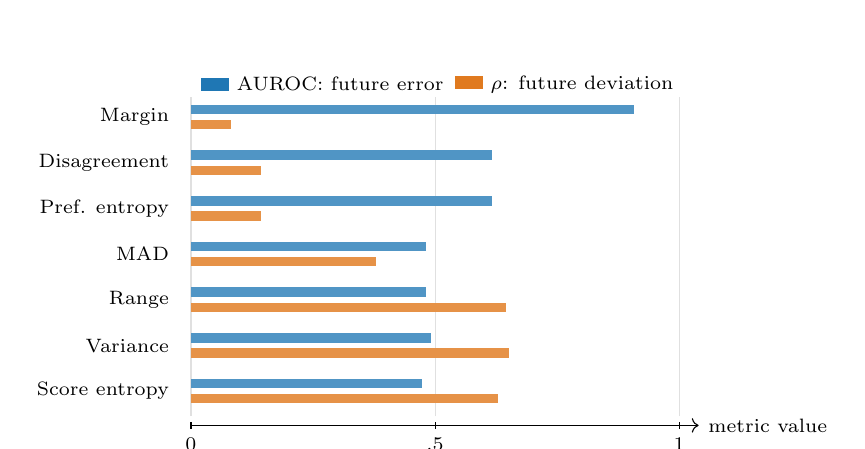
\begin{tikzpicture}[x=6.2cm,y=0.58cm,font=\scriptsize]
  \draw[->] (0,-0.75) -- (1.04,-0.75) node[right] {metric value};
  \foreach \x/\lab in {0/0,.5/.5,1/1} {
    \draw (\x,-0.82) -- (\x,-0.68) node[below=2pt] {\lab};
    \draw[black!12] (\x,-0.55) -- (\x,6.45);
  }
  \foreach \name/\y/\auc/\corr in {
    Margin/6/.908/.083,
    Disagreement/5/.617/.144,
    Pref. entropy/4/.617/.144,
    MAD/3/.481/.380,
    Range/2/.482/.645,
    Variance/1/.492/.652,
    Score entropy/0/.473/.628} {
    \node[anchor=east] at (-.025,\y) {\name};
    \fill[measureblue!78] (0,\y+.06) rectangle (\auc,\y+.27);
    \fill[uqorange!82] (0,\y-.27) rectangle (\corr,\y-.06);
  }
  \node[anchor=west] at (0,6.72) {\textcolor{measureblue}{\rule{1.3em}{0.6em}} AUROC: future error};
  \node[anchor=west] at (.52,6.72) {\textcolor{uqorange}{\rule{1.3em}{0.6em}} $\rho$: future deviation};
\end{tikzpicture}}
\caption{Signal--target ranking on validation.}
\end{subfigure}\hfill
\begin{subfigure}[t]{0.38\textwidth}
\centering
\resizebox{\linewidth}{!}{%
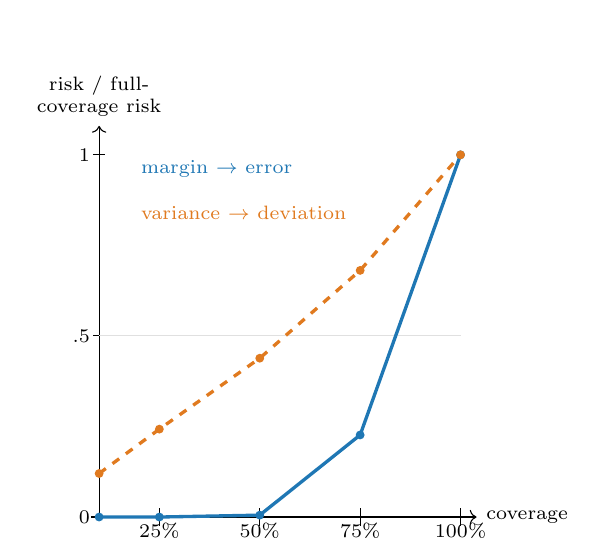
\begin{tikzpicture}[x=5.1cm,y=4.6cm,font=\scriptsize]
  \draw[->] (0.08,0) -- (1.04,0) node[right] {coverage};
  \draw[->] (0.10,0) -- (0.10,1.08) node[above,align=center] {risk / full-\\coverage risk};
  \foreach \x/\lab in {.25/25\%,.5/50\%,.75/75\%,1/100\%}
    \draw (\x,-.025) -- (\x,.025) node[below=2pt] {\lab};
  \foreach \y/\lab in {0/0,.5/.5,1/1}
    \draw (.085,\y) -- (.115,\y) node[left=2pt] {\lab};
  \draw[black!12] (.10,.5) -- (1,.5);
  \draw[very thick,measureblue] plot coordinates {
    (.10,0) (.25,0) (.50,.0052) (.75,.2266) (1,1)};
  \foreach \x/\y in {.10/0,.25/0,.50/.0052,.75/.2266,1/1}
    \fill[measureblue] (\x,\y) circle (1.6pt);
  \draw[very thick,uqorange,dashed] plot coordinates {
    (.10,.1202) (.25,.2427) (.50,.4385) (.75,.6809) (1,1)};
  \foreach \x/\y in {.10/.1202,.25/.2427,.50/.4385,.75/.6809,1/1}
    \fill[uqorange] (\x,\y) circle (1.6pt);
  \node[anchor=west,text=measureblue] at (.18,.96) {margin $\rightarrow$ error};
  \node[anchor=west,text=uqorange] at (.18,.84) {variance $\rightarrow$ deviation};
\end{tikzpicture}}
\caption{Validation risk--coverage.}
\end{subfigure}
\caption{Prospective UQ for the frozen winner.  Panel (a) compares all signals on
two distinct targets.  Panel (b) retains the lowest-uncertainty pairs within each of
252 complementary $5+5$ partitions and normalises risk by its full-coverage value.
Partitions are repeated views, not independent samples.  Plotted inputs are generated
by \texttt{scripts/generate\_dissertation\_figure\_data.py}.}
\label{fig:uq-signals-risk-coverage}
\end{figure}

\section{Risk--coverage interpretation}

AUROC summarises risk ranking but does not specify how a judge should act.  Sorting
pairs from low to high uncertainty yields a risk--coverage curve: coverage is the
fraction answered, and risk is error among answered pairs.  A useful UQ signal should
reduce risk as high-uncertainty pairs are withheld.  This principle underlies both
the APO failure-acquisition rule in \cref{chap:apo} and the adaptive inference policy
in \cref{chap:adaptive}.

In \cref{fig:uq-signals-risk-coverage}, retaining the least uncertain 50\% of pairs
reduces mean future reference error from $.0787$ at full coverage to $.00041$ under
margin uncertainty.  For the distinct continuous target, variance-ranked future
deviation falls from $.01698$ to $.00745$.  These curves are descriptive averages
over complementary partitions; inferential claims continue to be made at claim level.

\section{Chapter conclusion}

E6 provides a positive answer to RQ3 in the internal domain.  Black-box repeated
scores contain prospective information about future behaviour, and simple signals
are more useful than a single verbal confidence statement.  The strongest internal
signals are sampling variance for future deviation and margin uncertainty for future
error.  Their transfer is an empirical question, not an assumption.

% =============================================================================
\chapter{Uncertainty-Aware Automatic Prompt Optimisation}
\label{chap:apo}
% =============================================================================

\section{E7: optimisation paradigm}

The APO system performs discrete optimisation over readable instructions.  Task
definition, input fields, 0--100 scale, exact output format, Qwen target model, and
generation settings are frozen.  Only the instruction/rubric block can change.
Embeddings organise failure descriptions and prompt candidates; they are not learned
soft prompts and are not supplied as hidden vectors to the judge.

GPT-OSS-20B serves as the optimiser.  It receives the parent instruction and a
structured, diverse sample of Qwen failures, then proposes readable revisions.  Qwen
remains the only model that scores candidate prompts.  This separation prevents the
optimiser from directly determining evaluation outcomes.

\section{One search round}

The search used three rounds.  Each candidate was screened on 10 rotating,
stance-balanced APO-training claims using three seeds.  With four arguments, this is
$10\times4\times3=120$ score generations per candidate.  Three seeds are a cheap
screening proxy that distinguishes unanimous from 2--1 preferences; final UQ uses
ten runs.

One round executes the following loop:
\begin{enumerate}
  \item evaluate the population on a new training mini-batch;
  \item compute accuracy, normalised variance, flip rate, invalidity, tokens, and
  latency;
  \item prioritise wrong, tied, adjacent, high-dispersion, and seed-flipping pairs;
  \item convert failures to textual descriptions and embed them;
  \item cluster failures and select up to eight medoids;
  \item ask GPT-OSS for a structured critique and three readable rewrites per parent;
  \item embed candidate instructions and remove semantic near-duplicates;
  \item retain the Pareto set and rank candidates conservatively;
  \item repeat with the next rotating mini-batch.
\end{enumerate}

Failure clustering used cosine similarity threshold .72.  Candidate deduplication
used .92.  Embeddings came from
\texttt{sentence-transformers/all-MiniLM-L6-v2} at frozen revision
\texttt{1110a243\ldots b4d41}.  Optimiser generation used temperature .7, top-$p$
.95, and 2,048 maximum new tokens.

\section{Observed search trajectory}

\Cref{fig:apo-trajectory} exposes the complete candidate flow rather than reporting
only the selected prompt.  Four manual seed prompts entered round 0.  The optimiser
generated 12 rewrites; semantic filtering produced 15 candidates for round 1.  Four
round-1 survivors and eight non-duplicate rewrites produced 12 round-2 candidates;
the final round produced 15 candidates for promotion, of which two reached
validation.  The eventual winner first appeared among the round-0 rewrites.

\begin{figure}[htbp]
\centering
\resizebox{\textwidth}{!}{%
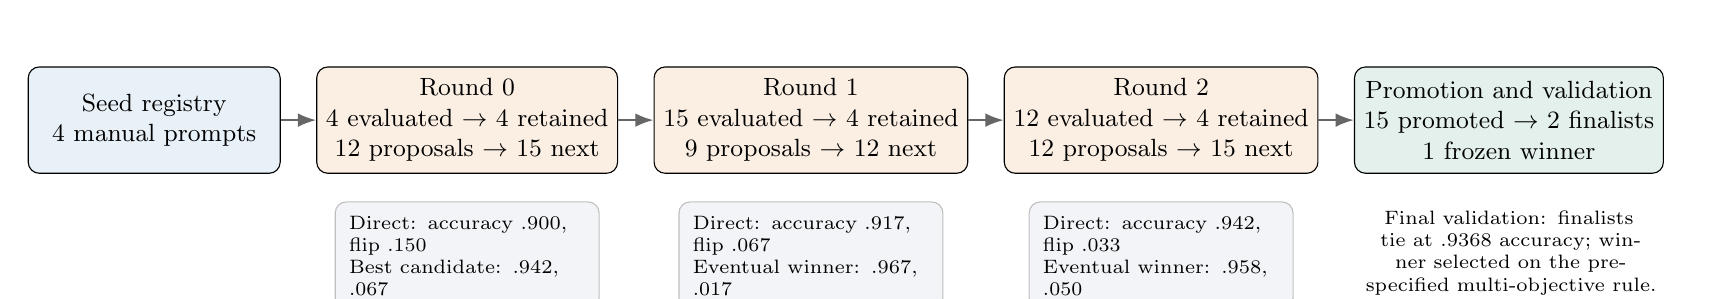
\begin{tikzpicture}[
  >=Latex,
  box/.style={draw,rounded corners,minimum width=3.2cm,minimum height=1.35cm,
    align=center,font=\small},
  arrow/.style={->,thick,draw=black!60},
  metric/.style={draw=black!25,fill=softgrey,rounded corners,align=left,
    text width=3.0cm,font=\scriptsize,inner sep=5pt}
]
\node[box,fill=measureblue!10] (seed) {Seed registry\\4 manual prompts};
\node[box,fill=uqorange!12,right=0.45cm of seed] (r0) {Round 0\\4 evaluated $\rightarrow$ 4 retained\\12 proposals $\rightarrow$ 15 next};
\node[box,fill=uqorange!12,right=0.45cm of r0] (r1) {Round 1\\15 evaluated $\rightarrow$ 4 retained\\9 proposals $\rightarrow$ 12 next};
\node[box,fill=uqorange!12,right=0.45cm of r1] (r2) {Round 2\\12 evaluated $\rightarrow$ 4 retained\\12 proposals $\rightarrow$ 15 next};
\node[box,fill=apogreen!13,right=0.45cm of r2] (promote) {Promotion and validation\\15 promoted $\rightarrow$ 2 finalists\\1 frozen winner};
\draw[arrow] (seed) -- (r0);
\draw[arrow] (r0) -- (r1);
\draw[arrow] (r1) -- (r2);
\draw[arrow] (r2) -- (promote);
\node[metric,below=0.35cm of r0] {Direct: accuracy .900, flip .150\\Best candidate: .942, .067};
\node[metric,below=0.35cm of r1] {Direct: accuracy .917, flip .067\\Eventual winner: .967, .017};
\node[metric,below=0.35cm of r2] {Direct: accuracy .942, flip .033\\Eventual winner: .958, .050};
\node[font=\scriptsize,align=center,text width=4.2cm,below=0.35cm of promote] {Final validation: finalists tie at .9368 accuracy; winner selected on the pre-specified multi-objective rule.};
\end{tikzpicture}}
\caption{APO candidate trajectory.  Counts come from the round manifests; metric
values come from each round's candidate summary.  Each round uses a different
rotating 10-claim batch, so cross-round point estimates are not a monotonic learning
curve.  The figure documents search and selection rather than claiming steady
improvement.}
\label{fig:apo-trajectory}
\end{figure}

\section{Multi-objective selection}

The implemented utility function supports candidate ranking from a conservative
accuracy lower bound
\begin{equation}
  \operatorname{LCB}(p)=\widehat p-1.96\operatorname{SE}(\widehat p)
\end{equation}
and subtracts penalties:
\begin{equation}
  J(p)=\operatorname{LCB}(p)-.15F(p)-.10V(p)-.10B(p)
  -.25I(p)-.02C(p),
  \label{eq:apo-objective}
\end{equation}
where $F$ is flip rate, $V$ normalised score variance, $B$ calibration error, $I$
invalid rate, and $C$ token excess beyond a 50-token budget.  Pareto filtering occurs
before scalar ranking, limiting the extent to which one favourable metric can hide a
dominated configuration.

Not every term was active at every stage.  During the three cheap screening rounds
no cross-fitted Brier estimate was available; the implementation assigned every
candidate the same fallback value $.25$, so $B$ cancelled from within-round ranking.
Moreover, mean completions were approximately six generated tokens, below the
50-token threshold, and the scalar cost penalty $C$ was therefore zero.  Generated
tokens and latency still entered the Pareto vector and could prevent dominance, but
\emph{mean tokens count completion tokens only}, not prompt-input tokens or monetary
cost.  The search-stage claim is consequently UQ-guided failure acquisition plus
accuracy--stability-aware selection, not active calibration optimisation or a
demonstrated scalar cost trade-off.

At validation, $B$ became active: it was the claim-cross-fitted Brier score from the
pre-specified sampling-variance signal.  The selected prompt's Brier was $.07799$
versus $.08527$ for the other finalist.  The token threshold remained inactive, so
the final decision combined the accuracy lower bound, flip rate, variance,
sampling-variance calibration, invalidity, and Pareto-level efficiency.  This
stage-specific account avoids attributing an optimisation effect to terms that were
only recorded or constant in the executed search.

\section{E8: successive halving and freezing}

Successive halving allocates more resources to fewer candidates
\cite{jamieson2016successive}.  The stages were fixed as shown in
\cref{tab:halving}.

\begin{table}[htbp]
\centering
\caption{E8 successive-halving stages.}
\label{tab:halving}
\begin{tabularx}{\textwidth}{lrrY}
\toprule
Stage & Claims & Seeds & Function \\
\midrule
Screening & 10 rotating train & 3 & Reject weak prompts and discover failures cheaply \\
Promotion & 30 train & 5 & Reduce survivors to two finalists \\
Full-training audit & 70 train & 5 & Diagnose robustness over all optimisation claims \\
Validation & 29 validation & 10 & Select exactly one prompt using UQ and utility \\
Internal test & 50 test & 10 & Evaluate frozen prompt once; no reselection \\
\bottomrule
\end{tabularx}
\end{table}

The two finalists tied on validation pairwise accuracy (.9368).  The selected prompt
had lower flip (.1264 versus .1839), lower normalised variance (.00134 versus .00161),
slightly fewer completion tokens, and higher pre-specified conservative utility
(.8722 versus .8611).  Prompt \texttt{p\_53a4acbe525c} was frozen before testing.  It asks the
judge to verify specificity, direct relevance, source credibility, and unsupported
generic statements.  Its exact text appears in \cref{app:prompts}.

\section{Full-training audit}

\begin{table}[htbp]
\centering
\caption{Paired comparison of the two finalists on all 70 training claims.  Positive
$\Delta$ favours the winner for accuracy; negative favours it for flip/variance.}
\label{tab:full-train}
\begin{tabular}{lrrrrrr}
\toprule
Metric & Winner & Finalist & $\Delta$ & 95\% CI & \rawp{} & \holmp{} \\
\midrule
Pairwise accuracy & .9476 & .9440 & .0036 & [-.0095,.0167] & .7252 & .7252 \\
Flip rate & .0619 & .0976 & -.0357 & [-.0667,-.0048] & .0388 & .0388 \\
Normalised variance & .000991 & .001188 & -.000197 & [-.000536,.000140] & .2570 & .2570 \\
\bottomrule
\end{tabular}
\end{table}

The finalists do not differ detectably in accuracy, but the selected prompt has a
significantly lower flip rate.  This audit is a robustness diagnostic on optimisation
data, not an independent estimate of generalisation.

\section{Frozen Qwen internal test}

\begin{table}[htbp]
\centering
\caption{Qwen internal-test summary on 50 claims and ten seeds.}
\label{tab:qwen-internal}
\begin{tabular}{lrrr}
\toprule
Prompt & Pairwise accuracy & Flip rate & Normalised variance \\
\midrule
Direct & .9067 & .1500 & .003137 \\
Role & .9483 & .1667 & .002584 \\
Rubric & .9367 & .1367 & .001030 \\
Role+Rubric & .9400 & .1233 & .001408 \\
\winner & .9417 & .0900 & .000942 \\
\bottomrule
\end{tabular}
\end{table}

The winner is competitive but not the highest point estimate for accuracy; Role is
.0067 higher.  Against Direct, the winner's +.035 accuracy contrast has raw
$p=.0434$ but does not survive Holm correction ($\holmp=.1736$).  The attack-only
accuracy advantage over Direct is larger (+.0761) and survives its declared family
($\holmp=.0078$).  Overall, the winner's main benefit is stability
(\cref{tab:qwen-internal-contrasts}).

The complete four-baseline comparison is essential.  Omitting Role or Role+Rubric
after observing the Main Study would make the internal result appear selectively
favourable.  The correct conclusion is successful multi-objective in-domain
optimisation: accuracy is competitive and Qwen repeated-run stability improves, but
the winner does not dominate every manual prompt.

\section{Cross-model Mistral audit}

\begin{table}[htbp]
\centering
\caption{Mistral transfer on the same 50 internal-test claims and ten seeds.}
\label{tab:mistral-transfer}
\begin{tabular}{lrrr}
\toprule
Prompt & Pairwise accuracy & Flip rate & Normalised variance \\
\midrule
Direct & .9183 & .2200 & .005477 \\
Rubric & .9200 & .2567 & .008956 \\
\winner & .9350 & .2933 & .013922 \\
\bottomrule
\end{tabular}
\end{table}

The winner's accuracy differences from Direct (+.0167, $\holmp=.4548$) and Rubric
(+.0150, $\holmp=.4548$) are not significant.  Its normalised variance is
significantly worse than Direct (+.00845, $\holmp=.00174$), and its flip-rate point
estimate is also worse.  The prompt text transfers syntactically, but the Qwen
stability advantage does not transfer as a reliability property.

\section{Chapter conclusion}

E7--E8 provide a qualified positive answer to RQ4.  The pipeline is an automatic
prompt optimisation algorithm: evaluation, uncertainty-aware failure acquisition,
embedding-based diversification, textual critique, rewriting, deduplication, and
selection form a repeated loop.  It finds a readable prompt with a strong Qwen
in-domain accuracy--stability profile.  The Mistral audit simultaneously demonstrates
why model-specific optimisation cannot be treated as universal prompt discovery.

% =============================================================================
\chapter{External Generalisation}
\label{chap:external}
% =============================================================================

Internal testing estimates generalisation within the primary dataset distribution.
E9 and E11 address RQ5 more strictly by using independent data and human quality
targets.  The winner remains frozen throughout.  External outcomes cannot trigger
rewriting, winner replacement, or calibration refitting.

\section{E9: IBM human-ranked external test}
\label{sec:e9}

\subsection{Design}

The formal E9 protocol evaluates Qwen3-8B with Direct, Role, Rubric, Role+Rubric, and
the frozen winner.  Generation is Hard, No-Think with ten seeds.  Thirteen formal
topics remain after two pilot topics are excluded.  Each topic--stance group supplies
a broad and a near-tie panel, producing 26 records per panel.  Human weighted-average
quality defines the reference order.

Inference is grouped by topic.  Confidence intervals use 10,000 topic-clustered
bootstrap resamples and p-values use 100,000 paired permutations.  Holm correction
is applied within each panel and metric.  The 5+5 UQ protocol uses all 252 partitions;
the validation-fitted isotonic mapping is transferred without external refitting.

\subsection{Prompt performance}

\begin{table}[htbp]
\centering
\caption{E9 overall accuracy and repeated-seed flip rate.}
\label{tab:e9-prompts}
\begin{tabular}{lrr}
\toprule
Prompt & Pairwise accuracy & Flip rate \\
\midrule
Direct & .524 [.452,.590] & .330 [.279,.381] \\
Role & .556 [.486,.623] & .391 [.340,.439] \\
Rubric & .574 [.521,.623] & .330 [.263,.401] \\
Role+Rubric & .559 [.503,.615] & .346 [.276,.429] \\
\winner & .540 [.492,.583] & .510 [.436,.587] \\
\bottomrule
\end{tabular}
\end{table}

No winner-versus-manual accuracy contrast reaches even unadjusted $p<.05$ in the
overall panel.  Against Rubric, for example, the winner difference is $-.0337$,
95\% CI $[-.0817,.0208]$, $\rawp=.2687$, and $\holmp=1.000$.
The winner is substantially less stable than every manual prompt; the complete
paired contrasts are reported in \cref{tab:e9-flip-tests} in the statistical
appendix.

Broad-panel accuracy is .583, .612, .622, .647, and .612 for Direct, Role, Rubric,
Role+Rubric, and the winner respectively.  Near-tie accuracy is .465, .500, .526,
.471, and .468.  Every prompt approaches chance on near-tie pairs; the broad panel is
more discriminable.  This mirrors the internal rank-distance analysis and shows that
boundary difficulty is not an artefact of the original reference construction.

\subsection{UQ transfer}

\begin{table}[htbp]
\centering
\caption{E9 UQ transfer for the frozen winner.  Calibration is transferred from
internal validation without refitting.}
\label{tab:e9-uq}
\begin{tabular}{lrrrr}
\toprule
Panel & Variance--deviation $\rho$ & Margin-error AUROC & Brier & ECE \\
\midrule
All pairs & .576 & .655 & .321 & .287 \\
Broad & .603 & .736 & .268 & .230 \\
Near tie & .555 & .564 & .374 & .350 \\
\bottomrule
\end{tabular}
\end{table}

Sampling variance remains positively associated with future deviation, and margin
uncertainty still ranks error above chance, especially in the broad panel.  However,
AUROC falls markedly from the internal value above .91, and the validation-fitted
probabilities are badly calibrated.  E9 therefore separates partial
\emph{risk-ranking transfer} from failed \emph{probability-calibration transfer}.

\section{E11: Webis-ArgQuality-20 replication}
\label{sec:e11}

\subsection{Design}

E11 tests whether the E9 result is specific to IBM ranking construction.  Qwen3-8B
uses Direct, Rubric, and the frozen winner under the same Hard, No-Think, ten-seed
protocol.  The formal test includes 18 topics, 36 topic--stance groups, and 4,925
majority-decisive human-labelled pairs.  Topics are the independent units.
The two confirmatory comparisons are winner versus Direct and winner versus Rubric;
Holm correction is applied within each scope and metric.

Pairwise accuracy gives a model tie half credit.  E11's exact directional accuracy
(reported as \emph{strict} in the result files) treats a predicted tie as wrong.  It
is not the Main Study's fixed ten-point strict-margin measure.

\subsection{Primary results}

\begin{table}[htbp]
\centering
\caption{E11 majority-decisive, topic-equal results.}
\label{tab:e11-summary}
\begin{tabular}{lrrrr}
\toprule
Prompt & Pairwise acc. & Exact direction & Flip rate & Norm. variance \\
\midrule
Direct & .5814 & .5343 & .2656 & .001182 \\
Rubric & .5892 & .5715 & .2995 & .000805 \\
\winner & .5979 & .5732 & .3782 & .000895 \\
\bottomrule
\end{tabular}
\end{table}

\begin{table}[htbp]
\centering
\caption{E11 winner-minus-baseline primary contrasts.}
\label{tab:e11-tests}
\begin{tabularx}{\textwidth}{llrrrr}
\toprule
Metric & Baseline & $\Delta$ & 95\% CI & \rawp{} & \holmp{} \\
\midrule
Pairwise accuracy & Direct & .0165 & [.0006,.0323] & .0671 & .1342 \\
Exact direction & Direct & .0389 & [.0145,.0646] & .00655 & .01310 \\
Flip rate & Direct & .1127 & [.0728,.1513] & .00010 & .00020 \\
Norm. variance & Direct & -.000287 & [-.000459,-.000127] & .00417 & .00834 \\
\addlinespace
Pairwise accuracy & Rubric & .0087 & [-.0045,.0218] & .2206 & .2206 \\
Exact direction & Rubric & .0018 & [-.0128,.0164] & .8135 & .8135 \\
Flip rate & Rubric & .0788 & [.0469,.1141] & .00021 & .00021 \\
Norm. variance & Rubric & .000090 & [.000014,.000161] & .0342 & .0342 \\
\bottomrule
\end{tabularx}
\end{table}

The pairwise bootstrap interval against Direct narrowly excludes zero while the
paired permutation p-value is .067.  This is not a contradiction: the interval and
test use different resampling constructions.  The pre-specified permutation test and
Holm family determine significance, so the pairwise contrast is reported as
borderline rather than significant.  Exact directional accuracy does improve over
Direct after correction, but not over Rubric.  The winner flips substantially more
often than both baselines.

Sensitivity analyses provide limited positive transfer.  On unanimously decisive
pairs, the winner reaches about .640 versus .616 for Direct and .617 for Rubric, but
adjusted pairwise contrasts remain non-significant.  On logically decisive pairs,
the pairwise advantage over Direct survives adjustment.  These results are
dimension- and baseline-conditional, not universal dominance.

\subsection{UQ replication}

\begin{table}[htbp]
\centering
\caption{E11 prospective UQ discrimination.}
\label{tab:e11-uq}
\begin{tabular}{lrrrrr}
\toprule
Prompt & Future error & Future flip & Var.--dev. $\rho$ & Margin AUROC & Disagree. AUROC \\
\midrule
Direct & .4729 & .0516 & .4599 & .6431 & .8170 \\
Rubric & .4355 & .0619 & .3353 & .5971 & .8258 \\
\winner & .4357 & .0764 & .3234 & .6223 & .7650 \\
\bottomrule
\end{tabular}
\end{table}

For the winner, the transferred calibration has Brier .3105 and ECE .2663.  UQ
signals retain moderate discrimination: sampling variance ranks future deviation,
margin uncertainty ranks human-reference error, and pair disagreement predicts
future model flips.  Nevertheless, internal probability calibration fails again.

\section{Combined external conclusion}

\begin{figure}[htbp]
\centering
\begin{subfigure}[t]{0.49\textwidth}
\centering
\resizebox{\linewidth}{!}{%
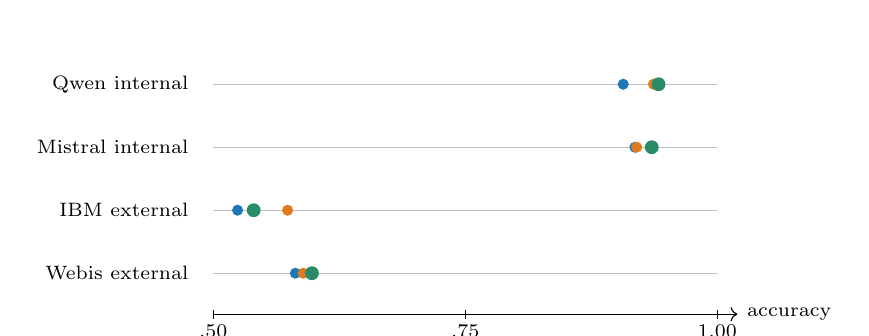
\begin{tikzpicture}[x=6.4cm,y=0.8cm,font=\scriptsize]
  \draw[->] (0,-.65) -- (1.04,-.65) node[right] {accuracy};
  \foreach \x/\lab in {0/.50,.5/.75,1/1.00}
    \draw (\x,-.72) -- (\x,-.58) node[below=2pt] {\lab};
  \foreach \name/\y/\dir/\rub/\win in {
    Qwen internal/3/.8134/.8734/.8834,
    Mistral internal/2/.8366/.8400/.8700,
    IBM external/1/.0481/.1474/.0801,
    Webis external/0/.1627/.1783/.1957} {
    \node[anchor=east] at (-.03,\y) {\name};
    \draw[black!25] (0,\y) -- (1,\y);
    \fill[measureblue] (\dir,\y) circle (2.0pt);
    \fill[uqorange] (\rub,\y) circle (2.0pt);
    \fill[apogreen] (\win,\y) circle (2.5pt);
  }
\end{tikzpicture}}
\caption{Pairwise accuracy.}
\end{subfigure}\hfill
\begin{subfigure}[t]{0.49\textwidth}
\centering
\resizebox{\linewidth}{!}{%
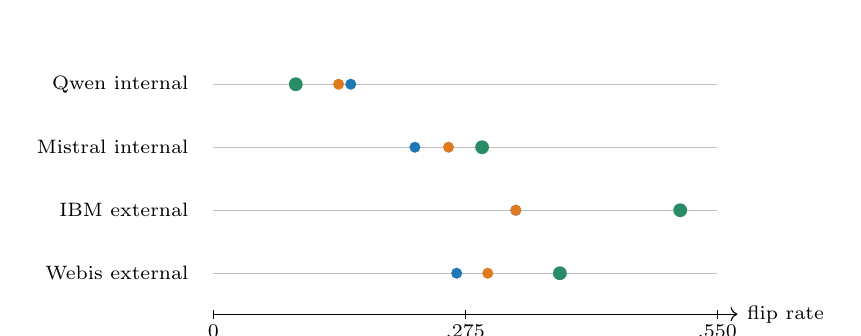
\begin{tikzpicture}[x=6.4cm,y=0.8cm,font=\scriptsize]
  \draw[->] (0,-.65) -- (1.04,-.65) node[right] {flip rate};
  \foreach \x/\lab in {0/0,.5/.275,1/.550}
    \draw (\x,-.72) -- (\x,-.58) node[below=2pt] {\lab};
  \foreach \name/\y/\dir/\rub/\win in {
    Qwen internal/3/.2727/.2485/.1636,
    Mistral internal/2/.4000/.4667/.5333,
    IBM external/1/.6002/.6002/.9265,
    Webis external/0/.4829/.5445/.6877} {
    \node[anchor=east] at (-.03,\y) {\name};
    \draw[black!25] (0,\y) -- (1,\y);
    \fill[measureblue] (\dir,\y) circle (2.0pt);
    \fill[uqorange] (\rub,\y) circle (2.0pt);
    \fill[apogreen] (\win,\y) circle (2.5pt);
  }
\end{tikzpicture}}
\caption{Repeated-seed flip rate.}
\end{subfigure}

\vspace{0.4em}
{\small\textcolor{measureblue}{\rule{1.2em}{0.65em}} Direct\quad
\textcolor{uqorange}{\rule{1.2em}{0.65em}} Rubric\quad
\textcolor{apogreen}{\rule{1.2em}{0.65em}} Frozen winner}
\caption{Transfer of prompt performance across the Qwen internal test, a cross-model
Mistral audit on the same claims, IBM-ArgQ-Rank-30k, and Webis-ArgQuality-20.
Within-domain comparisons are intended; absolute accuracy levels are not directly
comparable because the external datasets use different human constructs and pair
selection rules.  All three prompts use Hard, No-Think decoding and ten seeds.
Plotted inputs are generated by
\texttt{scripts/generate\_dissertation\_figure\_data.py}.}
\label{fig:accuracy-flip-transfer}
\end{figure}

The two external datasets support five conclusions.

\begin{enumerate}
  \item The internally selected prompt does not provide a robust external accuracy
  improvement over all manual baselines.
  \item Some accuracy effects transfer weakly or within particular quality scopes.
  \item The Qwen internal stability advantage reverses externally and under Mistral.
  \item Behavioural UQ signals retain partial risk-ranking information under shift.
  \item Validation-fitted probabilities do not remain calibrated without adaptation.
\end{enumerate}

External generalisation is therefore not a binary pass/fail property.  The prompt
text, accuracy effect, stability effect, risk ranking, and probability calibration
have different transfer behaviour.  The negative stability and calibration results
are substantive evidence about the boundary of in-domain optimisation.

% =============================================================================
\chapter{Adaptive Uncertainty-Aware Inference}
\label{chap:adaptive}
% =============================================================================

E10 addresses RQ6 by converting UQ from a diagnostic into a resource-allocation
policy.  The experiment is explicitly exploratory because its practical stopping
thresholds were examined after the main UQ/APO pipeline had been frozen.

\section{Policy design}

The frozen Qwen winner is calibrated on the 29 validation claims and evaluated on
the 50 internal-test claims, E9, and E11.  Up to ten stochastic runs are available.
A policy may stop after 3, 5, 7, or 10 runs.  It must report coverage, selective
accuracy, and mean runs together: accuracy among answered pairs can be increased
trivially by abstaining on almost everything.

\subsection{Bayesian stopping}

For a pair, the run-level outcomes are ``first argument preferred'', ``tie'', or
``second argument preferred''.  With counts
$\boldsymbol n=(n_A,n_T,n_B)$ and a symmetric prior
\begin{equation}
  \boldsymbol\pi\sim\operatorname{Dirichlet}(0.5,0.5,0.5),
\end{equation}
the posterior is
\begin{equation}
  \boldsymbol\pi\mid\boldsymbol n\sim
  \operatorname{Dirichlet}(n_A+0.5,n_T+0.5,n_B+0.5).
\end{equation}
At each checkpoint, the policy stops if the posterior confidence in the leading
direction exceeds $\tau\in\{.60,.70,.80,.90\}$; otherwise it allocates more runs.
At the final checkpoint it may answer or abstain, depending on whether the threshold
is met.  This is an empirical Bayesian policy and carries no distribution-free
coverage guarantee.

The implementation stores pairs in reference-oriented ``better/worse'' order for
evaluation convenience, but the stopping decision depends only on the maximum of the
three posterior category probabilities.  Relabelling the two arguments therefore
does not change when the policy stops.  Reference correctness is computed only after
the posterior decision has been made; it is not an outcome category available to a
deployed policy.

\subsection{Strict claim-grouped conformal rule}

A split-conformal alternative uses the validation claims to calibrate a
nonconformity score.  To seek simultaneous protection across every pair and
checkpoint in a claim, calibration takes the claim-level maximum.  Miscoverage
levels .05, .10, and .20 all produce threshold .9565 with only 29 calibration
claims.  The procedure is valid under its exchangeability assumptions, but the
maximum construction is highly conservative.

\section{Internal and E9 results}

\begin{table}[htbp]
\centering
\caption{Bayesian adaptive policy on the Qwen internal test.}
\label{tab:adaptive-internal}
\begin{tabular}{rrrrr}
\toprule
Threshold & Coverage & Selective pairwise acc. & Mean runs & Saving \\
\midrule
.60 & .987 & .943 & 4.0 & 60\% \\
.70 & .977 & .944 & 4.5 & 55\% \\
.80 & .953 & .958 & 6.5 & 35\% \\
.90 & .910 & .973 & 10.0 & 0\% \\
\bottomrule
\end{tabular}
\end{table}

Internally, thresholds .60--.80 preserve high coverage and save 35--60\% of the
ten-run budget.  A stricter threshold increases selective accuracy, but part of the
gain comes from withholding more pairs.

\begin{table}[htbp]
\centering
\caption{Bayesian adaptive policy on E9 overall.}
\label{tab:adaptive-e9}
\begin{tabular}{rrrrr}
\toprule
Threshold & Coverage & Selective pairwise acc. & Mean runs & Saving \\
\midrule
.60 & .811 & .573 & 7.23 & 27.7\% \\
.70 & .715 & .576 & 7.75 & 22.5\% \\
.80 & .628 & .579 & 9.42 & 5.8\% \\
.90 & .490 & .578 & 10.0 & 0\% \\
\bottomrule
\end{tabular}
\end{table}

E9 shows a weaker trade-off.  Increasing the threshold substantially reduces
coverage and saving without materially improving accuracy.  The policy detects
uncertainty but cannot repair a shifted human-reference relationship.

\section{E11 pair-at-a-time results}

\begin{table}[htbp]
\centering
\caption{Bayesian adaptive policy on E11 majority-decisive pairs.}
\label{tab:adaptive-e11}
\begin{tabular}{rrrrrr}
\toprule
Threshold & Coverage & Human acc. & Pairwise acc. & Mean runs & Saving \\
\midrule
.60 & .903 & .529 & .603 & 4.09 & 59.1\% \\
.70 & .834 & .545 & .608 & 4.51 & 54.9\% \\
.80 & .731 & .566 & .615 & 6.53 & 34.7\% \\
.90 & .623 & .586 & .622 & 10.0 & 0\% \\
\bottomrule
\end{tabular}
\end{table}

E11 again exhibits a usable cost--coverage curve, but the distinction between
selective human accuracy and tie-aware pairwise accuracy is important.  Higher
thresholds select cases on which the model is more internally decisive; that need not
imply proportionate agreement with human quality.

\section{Conformal result}

At every tested miscoverage level, the strict claim-grouped conformal rule abstains
on every internal and E9 pair.  Prediction-set coverage is 1.0, mean runs remain 10,
and computational saving is zero.  This is a valid but uninformative outcome under
the available calibration size and grouping rule.  It illustrates rather than
invalidates conformal prediction: a formal coverage guarantee can be too conservative
to provide operational utility.

\section{Chapter conclusion}

Adaptive sampling is useful when uncertainty is treated as a resource-allocation
signal.  Internally and on E11, moderate Bayesian thresholds save substantial
generation while preserving useful coverage.  E9 shows that adaptive sampling does
not overcome domain shift.  The conformal result exposes a guarantee--utility
trade-off: stronger simultaneous guarantees require more calibration data or a less
conservative problem formulation.

% =============================================================================
\chapter{Integrated Evaluation and Discussion}
\label{chap:evaluation}
% =============================================================================

\section{Answers to the research questions}

\begin{longtable}{@{}p{0.08\textwidth}p{0.84\textwidth}@{}}
\caption{Integrated answers to the research questions.}\label{tab:rq-answers}\\
\toprule
Question & Evidence-based answer \\
\midrule
\endfirsthead
\toprule
Question & Evidence-based answer \\
\midrule
\endhead
RQ1 &
The judges achieve high internal pairwise accuracy, but exact complete orders are
substantially harder and errors concentrate among adjacent arguments.  Manual prompt
effects are conditional on model and stance; no prompt is uniformly superior. \\
RQ2 &
Hard decoding guarantees format and reduces cost but can change model-dependent
score and stability behaviour.  Visible reasoning reduces Qwen ties but increases
dispersion and seed flips.  Protocol choices are part of the measurement. \\
RQ3 &
Yes, internally.  Sampling variance predicts future numerical deviation and inverse
margin predicts future order errors using disjoint 5+5 generations.  Internal
discrimination and calibration are strong. \\
RQ4 &
Partly.  UQ-aware APO finds a readable prompt with competitive Qwen accuracy and
lower internal flip than three manual baselines.  It does not dominate Role on
accuracy or Role+Rubric on flip, and its stability benefit is model-specific. \\
RQ5 &
Only conditionally.  The winner has limited E11 directional gains over Direct but no
robust advantage over Rubric.  Its internal stability benefit reverses on Mistral,
IBM, and Webis.  Risk ranking partially transfers; probability calibration does not. \\
RQ6 &
Bayesian adaptive sampling produces useful internal and E11 cost--coverage trade-offs
but cannot repair E9 domain shift.  The strict claim-level conformal rule is valid but
abstains everywhere with 29 calibration claims. \\
\bottomrule
\end{longtable}

\section{Reliability is multi-dimensional}

The results reject a one-number view of LLM-judge quality.  Five dimensions behave
differently:

\begin{description}
  \item[Accuracy] measures agreement with a reference ordering.
  \item[Repeatability] measures whether stochastic reruns preserve preferences.
  \item[Calibration] measures whether predicted risks match empirical frequencies.
  \item[Protocol robustness] measures sensitivity to prompt, decoding, reasoning,
  model, and data distribution.
  \item[Efficiency] measures the tokens, latency, and repetitions required.
\end{description}

A configuration can improve one dimension while worsening another.  Qwen Thinking
reduces ties but increases flips.  The APO winner reduces Qwen internal variance but
increases external flips.  Hard decoding improves validity and cost but can alter the
score distribution.  These are not contradictory outcomes; they show that the
measurement objectives are distinct.

\section{The protocol is part of the construct measurement}

The judge does not reveal a protocol-independent latent belief.  Prompt wording,
output restriction, reasoning mode, sampling, parsing, and aggregation jointly define
the operational measurement.  In particular, a 0--100 score cannot be assumed to
have a common interval meaning across models: the score-scale analysis shows
different ranges and digit heaping.  Rank-based comparisons are therefore more
defensible across models than a fixed raw-score margin.

This conclusion also explains why pointwise and pairwise should not be conflated.
The model generates pointwise scores, but reference agreement is evaluated pairwise.
Changing the displayed order of several candidates would test presentation-order
bias in a listwise judge; it is not the same as permuting independent pointwise calls.

\section{Boundary cases dominate difficulty}

Internal rank distance and E9 panel design converge on the same result.  Far-apart
arguments are easy; adjacent and near-tie arguments are difficult.  Aggregate
accuracy can therefore be inflated by the composition of pair difficulties.  Future
benchmarks should report accuracy by quality gap and should avoid treating all pairs
as equally informative.

Boundary cases are also where UQ is most necessary and most difficult.  Small margins
successfully locate risk internally, yet on E9 near ties all prompts are near chance
and margin-based AUROC approaches .5.  When the human reference itself is separated
by an extremely small quality gap, more model samples may estimate model preference
more precisely without making it align with humans.

\section{Risk ranking transfers better than calibration}

The UQ experiments expose a practically important distinction.  Sampling variance
and margin uncertainty remain directionally informative under dataset shift, but the
isotonic probabilities fitted on internal validation are badly miscalibrated
externally.  This is consistent with the general fact that calibration is
distribution-specific even when a score preserves useful ranking.

The appropriate external claim is therefore not that UQ fails or transfers
completely.  It is that \emph{risk ordering partially transfers, whereas absolute
risk probabilities require domain-specific recalibration}.  This distinction matters
for deployment: ranking cases for review may remain useful even when thresholds
based on nominal probabilities are unsafe.

\section{Automatic optimisation and overfitting}

The APO pipeline is algorithmic and reproducible, but it is still an optimiser of a
finite development distribution.  Its selected criteria---specificity, relevance,
source credibility, and avoidance of generic claims---fit important internal failure
clusters.  They do not guarantee that a different dataset encodes quality in the same
way.  E9 and E11 demonstrate that optimising stability on Qwen internal data can
produce a prompt whose external stochastic behaviour is worse.

This is not evidence that automatic prompt optimisation is pointless.  It specifies
what a stronger objective must include: multiple models, multiple domains, human
targets, and explicit distributionally robust penalties.  A readable prompt remains
valuable because its learned behaviour can be inspected; however, interpretability
of the instruction does not imply predictability of its transfer.

\section{Limitations}
\label{sec:limitations}

\subsection{Construct validity}

The primary four-argument reference orders are synthetic and may not always represent
a unique human consensus.  Manual audit identifies a small set of contestable pairs,
but the original labels are retained to avoid post-hoc relabelling.  IBM and Webis
provide stronger human-target evidence, yet operationalise quality differently.
This heterogeneity limits simple cross-dataset comparison while strengthening the
test of robustness.

\subsection{Internal holdout and adaptive development}

The 50-claim internal test was hidden from the APO algorithm, but earlier dissertation
analyses had used aggregate data from all 149 claims.  It is therefore an
algorithmically held-out test rather than a pristine project-level test.  E9 and E11
are the primary evidence for genuine external generalisation.

E10 is exploratory and its thresholds were not part of the earliest confirmatory
plan.  Its estimates describe available trade-offs but require new-data validation
before operational deployment.

\subsection{Models and sampling}

Only three open-weight model families were used, with Qwen as the principal UQ/APO
target.  Results may differ for larger proprietary judges, deterministic generation,
or alternative sampling temperatures.  Ten runs permit a prospective 5+5 design but
remain a small sample for complex multimodal score distributions.

\subsection{Statistical power and multiplicity}

Several effects are small relative to the number of independent claims or topics.
Holm correction reduces false positive risk but also widens the evidential threshold.
Both raw and adjusted p-values are reported so readers can inspect this trade-off.
Non-significant tests are not evidence of no effect, and failed equivalence tests
show that some intervals remain too wide to exclude practically relevant differences.

\subsection{Calibration and conformal sample size}

Isotonic regression is flexible and can overfit small calibration samples even under
cross-fitting.  The external calibration failure demonstrates this limitation.
Similarly, 29 validation claims are insufficient for a useful strict maximum-over-
pairs conformal threshold.  Pair-level conformal calibration would be less
conservative but would not provide the same simultaneous claim-level guarantee.

\subsection{Cost measurement}

Latency was measured on the available cluster hardware and includes model- and
system-specific effects.  Token counts are more portable than wall-clock seconds,
but even tokens are not a direct monetary or energy measure.  The report therefore
uses latency and tokens as operational indicators rather than universal cost units.

\section{Ethical and reproducibility considerations}

No new human participants were recruited.  External targets come from previously
released argument-quality datasets and are used under their stated licences.
Arguments may contain sensitive or contentious claims; model errors should not be
interpreted as authoritative conclusions about those claims.  An LLM judge should
not replace human oversight in high-stakes deliberation.

Reproducibility is supported through pinned model revisions, deterministic data
fingerprints, locked split and freeze manifests, raw JSONL generations, processed CSV
tables, and analysis scripts.  Invalid outputs are retained as invalid rather than
silently imputed.  Pilot topics are excluded from formal external tests.  The
repository structure and reproduction commands are summarised in
\cref{app:reproducibility}.

% =============================================================================
\chapter{Conclusions and Future Work}
\label{chap:conclusion}
% =============================================================================

\section{Conclusions}

This dissertation investigated LLM-based argument-strength judgement as a stochastic
measurement problem.  The initial studies showed that high aggregate pairwise
accuracy coexists with difficult adjacent comparisons, lower exact-order accuracy,
model-specific prompt effects, score-scale incompatibility, and sensitivity to
decoding and visible reasoning.  These findings motivated a prospective UQ protocol
rather than continued manual prompt refinement.

Repeated sampling proved informative internally.  Variance predicts how much future
scores will move, and inverse margin predicts whether future ordering will be wrong.
Embedding-assisted UQ-aware APO then used those signals to identify representative
failures and optimise readable prompt text.  The selected prompt produced a strong
Qwen internal accuracy--stability profile, but external evaluation was decisive: the
stability improvement did not transfer, and calibrated probabilities degraded
sharply.  A second external dataset provided limited accuracy transfer over Direct
but no dominance over Rubric and again showed worse seed stability.

The project therefore succeeds without discovering a universally best prompt.  Its
main result is a more defensible account of reliability:
\begin{quote}
An LLM judge is reliable only relative to a model, prompt, decoding and sampling
protocol, target construct, and data distribution; accuracy, stability, calibration,
and cost must be evaluated jointly.
\end{quote}

\section{Practical recommendations}

For the studied setting:

\begin{enumerate}
  \item use a simple Direct or explicit Rubric baseline before investing in complex
  manual prompting;
  \item use hard decoding when exact score validity and low cost are essential, but
  validate its measurement effect for the target model;
  \item do not interpret fewer ties or a longer rationale as calibrated certainty;
  \item repeat stochastic scoring and report dispersion or pair disagreement;
  \item use margin and variance to prioritise review, but recalibrate risk after
  domain shift;
  \item validate an optimised prompt on every intended model and domain;
  \item report selective accuracy together with coverage and sampling cost.
\end{enumerate}

\section{Future work}

\subsection{Distributionally robust APO}

A stronger search objective would evaluate every candidate across multiple models
and human-labelled domains, optimising worst-domain or distributionally robust
utility rather than one Qwen development split.  Domain-balanced acquisition could
ensure that failure medoids cover different datasets and quality dimensions.

\subsection{Hierarchical Bayesian UQ}

A hierarchical model could separate uncertainty attributable to claims, arguments,
models, prompts, and stochastic runs.  Partial pooling would improve estimates for
small groups and produce posterior predictive risk for new claims.  Such a model
would be a genuine extension beyond the current empirical Dirichlet stopping rule.

\subsection{Domain-adaptive calibration}

External results motivate calibration transfer methods: small labelled calibration
sets, covariate-aware recalibration, importance weighting, or online calibration.
Evaluation should distinguish improved Brier/ECE from preserved AUROC and should use
new topics after adaptation.

\subsection{Boundary-aware evaluation}

Future acquisition can oversample adjacent and human-near-tie pairs while retaining
a broad control panel.  A useful benchmark would report performance as a continuous
function of human quality gap and allow an explicit indifference region where no
unique strict order is defensible.

\subsection{Set-valued ranking and abstention}

Rather than forcing a total order, the judge could return partial orders or
set-valued ranks when uncertainty is high.  Larger calibration sets would enable less
degenerate conformal constructions.  The target should be a useful joint guarantee
over rank sets, coverage, and computational cost.

\subsection{Joint prompt and inference-policy optimisation}

The current pipeline optimises prompt text first and inference policy later.  A
future algorithm could jointly choose the instruction, number of samples, aggregation
rule, and abstention threshold.  Its objective should include human accuracy,
stability, calibration, coverage, and energy or latency cost under a fixed budget.

\section{Final statement}

The most useful outcome of the work is not a single winning prompt.  It is an
experimental framework that makes hidden uncertainty observable, incorporates it
into optimisation, and then subjects the apparent gain to locked internal and
external falsification.  That progression---measurement, quantification, mitigation,
and transfer---provides a stronger basis for trustworthy LLM-based evaluation than
one-shot accuracy alone.

% =============================================================================
% REFERENCES AND DECLARATIONS ARE UNNUMBERED, AS REQUIRED
% =============================================================================

\clearpage
\phantomsection
\addcontentsline{toc}{chapter}{References}
\renewcommand{\bibname}{References}
\bibliographystyle{unsrtnat}
\bibliography{references}

\clearpage
\chapter*{Declarations}
\addcontentsline{toc}{chapter}{Declarations}

\section*{Declaration of originality}

I declare that this report is my own work, except where the work of others is
acknowledged through citation.  The experimental results reported here were produced
from the code, configurations, datasets, and model generations identified in the
project repository.  I take responsibility for the experimental design, verification
of the reported numbers, interpretation, and final submitted text.

\section*{Use of generative artificial intelligence}

I acknowledge the use of OpenAI Codex, GPT-5 family (OpenAI,
\url{https://openai.com/codex/}, accessed August 2026), for structured feedback on
report organisation, British-English language editing, LaTeX and code suggestions,
debugging assistance, and generation of analysis/figure scaffolding.  It was not
treated as an evidential source.  Suggestions were checked against the cited
literature, source code, frozen manifests, and machine-readable result tables and
were revised or rejected where necessary.  I determined the research questions,
approved and ran the experiments, checked the analyses and citations, and remain
responsible for the submitted work.

Qwen3-8B, Mistral-7B-Instruct, and GPT-OSS-20B also appear as experimental objects or
algorithmic components.  Those uses are reported in the methodology and are distinct
from the authoring assistance declared above.  This disclosure follows Imperial
College London's Library guidance that the tool, publisher, URL, purpose, and the
author's responsibility should be stated.

\section*{Ethics and data}

The project did not recruit new human participants.  It uses existing argument
datasets and open-weight language models subject to their source licences and terms.
IBM-ArgQ-Rank-30k and Webis-ArgQuality-20 contain previously released human
annotations; this project analyses those existing labels and does not attempt to
identify annotators.  Arguments may concern contentious topics, so model scores are
research measurements rather than endorsements or professional, legal, medical, or
political advice.

\section*{Sustainability}

Repeated stochastic generation and three open-weight model families require material
GPU compute.  The implementation reduces avoidable repetition through checkpointed
JSONL output, resumable stages, successive halving, and short hard-constrained score
generation where the design permits it.  Completion tokens and latency are reported
as operational proxies, but cluster energy and carbon intensity were not metered;
the report therefore makes no quantitative environmental-impact claim.

\section*{Availability of data and materials}

Source code, configuration files, split and freeze manifests, raw model generations,
processed tables, and figure-data derivations accompany the project repository.
Third-party datasets and model weights remain subject to their original licences and
distribution terms.  The primary synthetic dataset's available provenance and its
missing upstream generation/verification records are disclosed in
\cref{sec:data-governance}; E9 and E11 dataset revisions and fingerprints are listed
in \cref{app:data-locks}.

% =============================================================================
% APPENDICES
% =============================================================================

\appendix

\chapter{Exact Prompt Instructions}
\label{app:prompts}

This appendix records the text that varied between experimental conditions.
The claim and argument were inserted at run time.  Line breaks shown here were
preserved by the implementation.

\section{Frozen task and response scale}

The following task and response block was common to every manual condition and
every APO candidate:

\begin{quote}\small
Evaluate the strength of the argument in performing its stated role with respect
to the claim.

\texttt{Claim: <claim>}\\
\texttt{Role: The argument is intended to <support/attack> the claim.}\\
\texttt{Argument: <argument>}

Assign an integer score from 0 to 100, where 0 means the argument provides no
valid or effective reason for its stated role, and 100 means the argument
provides an exceptionally strong and effective reason for its stated role.

Respond with exactly: \texttt{Score: <integer>}
\end{quote}

In hard-decoding conditions the response space was additionally restricted to
the 101 complete strings \texttt{Score: 0}, \ldots, \texttt{Score: 100}.

\section{Manual prompt conditions}

The design was a controlled $2\times2$ factorial intervention: the Role factor
added a persona instruction and the Rubric factor added explicit criteria.

\paragraph{Direct.}
No additional instruction was inserted between the task and response scale.

\paragraph{Role.}
\begin{quote}\small
You are an impartial expert analyst in argumentation. Assess arguments
consistently and do not favour supporting or attacking arguments.
\end{quote}

\paragraph{Rubric.}
\begin{quote}\small
Assess the argument using the following criteria:
\begin{enumerate}
  \item Factuality: Are its factual statements accurate and credible?
  \item Relevance: Does it directly address the claim?
  \item Logical quality: Does its reasoning justify its intended conclusion?
  \item Effectiveness: How strongly does it perform its stated supporting or
        attacking role?
\end{enumerate}
For a supporting argument, a strong argument should provide valid reasons that
the claim is true or credible.  For an attacking argument, the corresponding
rule states that a strong argument should provide valid reasons that the claim
is false, doubtful, or less credible.

Give one holistic score. Do not output separate criterion scores.
\end{quote}

\paragraph{Role+Rubric.}
The Role block was placed before the common task, and the Rubric block after the
task.  No other task or output wording changed.

\section{Frozen APO winner}

The validation-selected candidate had identifier
\texttt{p\_53a4acbe525c}.  Its optimised instruction block was:

\begin{quote}\small
Evaluate each reference by verifying:
\begin{itemize}
  \item \textbf{Specificity} --- does it provide direct facts, data, or
        concrete examples that address the claim?
  \item \textbf{Relevance} --- is the evidence directly linked to the claim or
        merely tangential?
  \item \textbf{Source credibility} --- is the reference from a reputable,
        verifiable source?
  \item Avoid generic statements such as \emph{many people believe} or
        \emph{it is known} unless a reliable source backs them.
\end{itemize}
References that fail these checks should lower the argument's score.  The
stance-specific relation rule from the common template follows this block.
\end{quote}

The wording refers to \emph{references} because it was generated from clustered
failure cases by the optimiser.  It remained frozen after validation; neither
internal-test nor external results were used to edit it.


\chapter{Hyperparameters and Experiment Inventory}
\label{app:hyperparameters}

\section{Common generation settings}

Unless a study explicitly varied decoding or reasoning, generation used hard
decoding, No-Think mode, stochastic sampling, temperature $0.7$, nucleus
parameter $p=0.95$, repetition penalty $1.0$, and a maximum of 12 newly
generated tokens.  The target models were Qwen3-8B, Mistral-7B-Instruct, and
GPT-OSS-20B as specified per study.  GPT-OSS-20B served as the text optimiser
in E7; Qwen3-8B remained the scored target model in the primary APO/UQ pipeline.

The common seed sequence was 42, 1024, 2026, 31415, 27182, 16180, 57721,
65537, 99991, and 104729.  Three-seed experiments used the first three values;
five-seed experiments used the first five.  In prospective UQ, the first five
runs formed an estimate set and the remaining five formed a disjoint held-out
set.  Analyses over all five-versus-five partitions used all
$\binom{10}{5}=252$ complementary views without treating them as independent
datasets.

\section{Complete experiment inventory}

\begin{longtable}{@{}p{0.07\textwidth}p{0.18\textwidth}p{0.52\textwidth}p{0.13\textwidth}@{}}
\caption{Experiments included in, or explicitly excluded from, the final report.}
\label{tab:appendix-inventory}\\
\toprule
ID & Study & Configuration and purpose & Status \\
\midrule
\endfirsthead
\toprule
ID & Study & Configuration and purpose & Status \\
\midrule
\endhead
E0 & Output-length pilots & 10 claims; Qwen and GPT-OSS; soft decoding;
Think/No-Think.  Established token ceilings and truncation diagnostics. & Complete \\
E1 & Decoding validation & 20 claims (10 support, 10 attack); three models;
Rubric; Hard/Soft; No-Think; three seeds. & Complete \\
E2 & Main Study & 149 claims, four arguments each; three models; four manual
prompts; Hard; No-Think; three seeds. & Complete \\
E3 & Reasoning Study & 50 claims (25 support, 25 attack); Qwen and GPT-OSS;
four prompts; Soft; Think/No-Think; three seeds. & Complete \\
E4 & Representation sensitivity & Expanded/synonym-derived version of the
149-claim data; planned three models, Rubric, Hard, No-Think. & Not run \\
E5 & Locked design & Claim-disjoint 70/29/50 APO-train/validation/internal
split; stance-balanced; fingerprinted before search. & Complete \\
E6 & Prospective UQ & Qwen; Hard; No-Think; ten runs; disjoint five-run
estimate and held-out sets; ranking, calibration, and risk--coverage metrics. & Complete \\
E7 & UQ-aware APO & Three search rounds; four-candidate population; rotating
10-claim screens with three seeds; failure clustering and GPT-OSS rewrites. & Complete \\
E8 & Successive halving & 30-claim promotion with five seeds; 70-claim audit
with five; 29-claim validation and 50-claim test with ten. & Complete \\
E9 & IBM external test & 13 untouched formal topics; 52 four-argument panels;
five prompts; Qwen; ten seeds; human weighted-average ranks. & Complete \\
E10 & Adaptive UQ & Post-freeze Dirichlet/Bayesian stopping at 3, 5, 7, or 10
runs and a strict claim-level conformal abstention analysis. & Complete; exploratory \\
E11 & Webis replication & 18 formal topics; direct human pair labels; Direct,
Rubric, and frozen winner; Qwen; ten seeds. & Complete \\
\bottomrule
\end{longtable}

\section{APO search and selection hyperparameters}

The APO search used three rounds, population size four, three proposals per
parent, eight representative failures, a failure-cluster similarity threshold
of 0.72, and a candidate near-duplicate threshold of 0.92.  Failure and
candidate texts were embedded with
\texttt{sentence-transformers/all-MiniLM-L6-v2} at revision
\texttt{1110a243fdf4706b3f48f1d95db1a4f5529b4d41}.  The generic utility
implementation used a 1.96-standard-error accuracy lower bound and weights of 0.15
for flip rate, 0.10 for normalised variance, 0.10 for Brier score, 0.25 for
invalidity, and 0.02 for generated-token excess beyond a 50-token budget.  In
screening, Brier was the same fallback value for every candidate and all completions
were below the token threshold, so those two scalar terms were inactive; tokens and
latency still entered Pareto dominance.  On validation, the Brier term used
claim-cross-fitted sampling-variance calibration, while the token penalty remained
zero.  The weights were not fitted on internal-test or external outcomes.

External analyses used 10,000 topic-clustered bootstrap resamples and 100,000
paired sign-flip/permutation resamples with analysis seed 42.  The E10 adaptive
policy used a symmetric Dirichlet prior concentration of 0.5 and posterior
confidence thresholds 0.60, 0.70, 0.80, and 0.90.


\chapter{Supplementary Statistical Results}
\label{app:statistics}

\section{Multiplicity and interpretation of significance}

The report gives exact two-sided raw and Holm-adjusted $p$-values for its key
families of prompt contrasts.  Holm correction was performed within each
predefined model, scope, and metric family.  This controls the family-wise
error rate while retaining more power than a simple Bonferroni division.  Raw
$p$-values are retained for transparency and exploratory interpretation, but a
raw value below 0.05 is not presented as confirmatory when the adjusted value
exceeds 0.05.  Confidence intervals and effect direction are interpreted
alongside $p$-values; statistical non-significance is not equated with proof of
no effect.

\section{Detailed prompt contrasts moved from the main chapters}

\begin{table}[htbp]
\centering
\caption{Selected E2 attack-stance contrasts that survive Holm correction.  The
difference is left prompt minus right prompt.}
\label{tab:e2-conditional}
\begin{tabularx}{\textwidth}{llYrrrr}
\toprule
Model & Metric & Contrast & $\Delta$ & 95\% CI & \rawp{} & \holmp{} \\
\midrule
GPT-OSS & Spearman & Role+Rubric $-$ Role & .0803 & [.0355,.1257] & .00050 & .0110 \\
GPT-OSS & Pairwise acc. & Role+Rubric $-$ Role & .0560 & [.0274,.0833] & .00040 & .0092 \\
GPT-OSS & Strict acc. & Role+Rubric $-$ Role & .0920 & [.0473,.1368] & .00030 & .0072 \\
Mistral & Spearman & Rubric $-$ Direct & .0570 & [.0244,.0948] & .0010 & .0210 \\
Mistral & Pairwise acc. & Rubric $-$ Direct & .0423 & [.0211,.0647] & .00040 & .0088 \\
\bottomrule
\end{tabularx}
\end{table}

\begin{table}[htbp]
\centering
\caption{Winner-minus-baseline Qwen internal-test contrasts.}
\label{tab:qwen-internal-contrasts}
\begin{tabularx}{\textwidth}{llrrrr}
\toprule
Metric & Baseline & $\Delta$ & 95\% CI & \rawp{} & \holmp{} \\
\midrule
Accuracy & Direct & .0350 & [.0017,.0650] & .0434 & .1736 \\
Accuracy & Role & -.0067 & [-.0383,.0200] & .7572 & 1.000 \\
Accuracy & Rubric & .0050 & [-.0167,.0283] & .7752 & 1.000 \\
Accuracy & Role+Rubric & .0017 & [-.0300,.0317] & 1.000 & 1.000 \\
\addlinespace
Flip rate & Direct & -.0600 & [-.1100,-.0133] & .0240 & .0481 \\
Flip rate & Role & -.0767 & [-.1233,-.0267] & .0047 & .0187 \\
Flip rate & Rubric & -.0467 & [-.0767,-.0133] & .0092 & .0277 \\
Flip rate & Role+Rubric & -.0333 & [-.0700,.0033] & .1085 & .1085 \\
\bottomrule
\end{tabularx}
\end{table}

\begin{table}[htbp]
\centering
\caption{E9 winner-minus-baseline flip-rate contrasts.  Positive values mean that
the winner flips more often.}
\label{tab:e9-flip-tests}
\begin{tabular}{lrrrr}
\toprule
Baseline & $\Delta$ flip & 95\% CI & \rawp{} & \holmp{} \\
\midrule
Direct & .1795 & [.0929,.2756] & .00284 & .01136 \\
Role & .1186 & [.0417,.1891] & .01543 & .04422 \\
Rubric & .1795 & [.0673,.2821] & .01474 & .04422 \\
Role+Rubric & .1635 & [.0545,.2660] & .01954 & .04422 \\
\bottomrule
\end{tabular}
\end{table}

\section{Complete prospective UQ comparison}

\begin{table}[htbp]
\centering
\caption{All validation UQ signals for the frozen winner, averaged over 252
complementary $5+5$ partitions.  Spearman predicts future absolute deviation;
AUROC/AUPRC/Brier/ECE use future reference error.  Partitions are not independent.}
\label{tab:uq-all-signals}
\begin{tabular}{lrrrrrr}
\toprule
Signal & $\rho$ & AUROC & AUPRC & AURC & Brier & ECE \\
\midrule
Margin uncertainty & .0827 & .9076 & .6079 & .01384 & .0557 & .0446 \\
Pair disagreement & .1439 & .6172 & .2483 & .01683 & .0726 & .0213 \\
Preference entropy & .1439 & .6172 & .2483 & .01683 & .0726 & .0213 \\
Sampling MAD & .3798 & .4811 & .1334 & .01498 & .0750 & .0134 \\
Sampling range & .6449 & .4818 & .1487 & .00828 & .0767 & .0187 \\
Sampling variance & .6521 & .4915 & .1352 & .00805 & .0780 & .0208 \\
Score-option entropy & .6283 & .4727 & .0897 & .00868 & .0743 & .0195 \\
\bottomrule
\end{tabular}
\end{table}

\section{APO search trajectory}

\begin{table}[htbp]
\centering
\caption{Executed APO trajectory.  ``Proposals'' is the raw rewrite count before
semantic deduplication.  Metrics are not compared as a learning curve because the
screening claims rotate.}
\label{tab:apo-search-trajectory}
\begin{tabular}{lrrrrrrr}
\toprule
Round & Eval. & Keep & Proposals & Next & Direct acc./flip & Best acc./flip & Winner acc./flip \\
\midrule
0 & 4 & 4 & 12 & 15 & .900/.150 & .942/.067 & -- \\
1 & 15 & 4 & 9 & 12 & .917/.067 & .967/.017 & .967/.017 \\
2 & 12 & 4 & 12 & 15 & .942/.033 & .958/.033 & .958/.050 \\
\bottomrule
\end{tabular}
\end{table}

\section{Equivalence tests}

Two one-sided equivalence tests used practical bounds of $\pm0.02$ for pairwise
accuracy and $\pm0.03$ for Spearman correlation.  No prompt contrast satisfied
both one-sided requirements after within-model Holm correction.  The defensible
conclusion is therefore that the study detected no robust universal prompt
improvement and also lacked sufficient precision to establish that all complex
prompts were practically equivalent to Direct.

\section{Score-scale diagnostics}

All three judges discretised the nominal 0--100 scale.  Approximately 71\% of
GPT-OSS scores, 79\% of Mistral scores, and 49\% of Qwen scores were multiples
of ten.  Mean within-claim ranges were approximately 47.9 for GPT-OSS and 79
for Mistral and Qwen.  Consequently, a fixed ten-point \emph{strict} margin does
not represent the same relative separation for every model.  Rank-based
accuracy is the principal cross-model endpoint; strict accuracy is interpreted
as a model-scale-dependent sensitivity measure.

\section{Tie-transition diagnostic}

Among 66 Qwen No-Think mean-tied pairs, Thinking produced a correct direction
for 49, a wrong direction for nine, and retained a tie for eight.  However,
39 of the 66 cases disagreed in direction across Thinking seeds, and 21 showed
both correct and wrong directions.  These transitions support a mechanistic
claim about decisiveness, not a claim that chain-of-thought reliably resolves
epistemic uncertainty.

\section{Machine-readable result tables}

The principal tables in the report are derived from the following directories:
\begin{itemize}
  \item \texttt{results/processed/main\_study/} for E2 prompt contrasts;
  \item \texttt{results/processed/reasoning\_study/} and
        \texttt{results/processed/extended\_analysis/} for E3 and analyses A--F;
  \item \texttt{results/uq\_apo/processed/} for E6--E10;
  \item \texttt{results/uq\_apo/processed/e11\_webis/} for E11.
\end{itemize}
The CSV files, rather than rounded prose values, are the auditable source for
all reported statistics.


\chapter{Data Locks, Splits, and Fingerprints}
\label{app:data-locks}

\section{Internal development split}

The internal source dataset contains 149 claims and has SHA-256 fingerprint
\texttt{5710a2cfa45789f138c89f76ead7bc7b62f99e6a4d85e278e23cbd8edaad877b}.
Split seed 20260802 produced 70 APO-training claims (39 support, 31 attack),
29 validation claims (16 support, 13 attack), and 50 internal-test claims
(27 support, 23 attack).  Claim identifiers do not overlap.  The complete ID
lists are stored in \texttt{configs/splits/uq\_apo\_claim\_splits.json}.

This lock prevents algorithmic leakage during E7--E8.  It is not a pristine
holdout relative to the entire dissertation because earlier E2 analyses had
already summarised all 149 claims.  The report therefore reserves its strongest
generalisation language for E9 and E11.

\section{E9 external lock}

E9 uses the official IBM Argument Quality Ranking 30k test split at revision
\texttt{590726b3765b1b90c5e53a17e3b1f77d92d3aa8a}.  The source CSV fingerprint
is \texttt{18c0f0491e0206558f24dbe79b91901bd662e5ec2b1bd9d13ab740660b0c196f}.
Two deterministically selected pilot topics were excluded.  The formal 52-record
file has fingerprint
\texttt{e77fd9fb9eb790ad993c8931e48733046b63f14fe934c85a885bc95600edda4e}.

\section{E11 external lock}

E11 uses Webis-ArgQuality-20 version 1.0.0.  Eighteen formal topics remained
after two deterministic pilot topics were excluded.  The formal generation
file and pair file have fingerprints
\texttt{f8475c93f8b4e8186d02942b13e95560e937bad1fb96a9e7bda8ffa4e2ea10ee}
and
\texttt{7803216a536d736f0e2a2a598b6e3191a69966234f44bafceb537917338f6ec8},
respectively.  Only valid, same-topic, same-stance argument pairs enter the
primary majority-decisive analysis.


\chapter{Reproducibility Guide}
\label{app:reproducibility}

This appendix gives an execution map rather than source-code listings.  It is
intended to connect each result to repository artefacts while leaving code in
the accompanying repository, as required for the project report.

\section{Configuration and implementation map}

\begin{longtable}{@{}p{0.27\textwidth}p{0.66\textwidth}@{}}
\toprule
Purpose & Repository artefacts \\
\midrule
Manual prompts and output format & \texttt{src/argstrength/prompts.py},
\texttt{src/argstrength/constraints.py}, \texttt{src/argstrength/parsing.py} \\
Locked UQ/APO protocol & \texttt{configs/uq\_apo.yaml},
\texttt{configs/splits/uq\_apo\_claim\_splits.json} \\
UQ estimators & \texttt{src/argstrength/uq.py},
\texttt{scripts/analyse\_uq.py} \\
APO loop & \texttt{src/argstrength/apo.py},
\texttt{src/argstrength/optimizer\_model.py},
\texttt{scripts/run\_prompt\_optimization.py} \\
Stage evaluation & \texttt{scripts/run\_apo\_stage.py},
\texttt{scripts/analyse\_apo\_stage.py} \\
IBM external test & \texttt{configs/e9\_external.yaml} and the E9 preparation,
generation, and analysis scripts under \texttt{scripts/} \\
Webis external test & \texttt{configs/e11\_webis\_external.yaml} and the E11
preparation, generation, and analysis scripts under \texttt{scripts/} \\
Adaptive inference & \texttt{configs/bayesian\_adaptive.yaml},
\texttt{src/argstrength/bayesian\_adaptive.py} \\
Dissertation figure inputs &
\texttt{scripts/generate\_dissertation\_figure\_data.py} and
\texttt{results/figures/dissertation/} \\
\bottomrule
\end{longtable}

\section{Execution order}

The reproducible order is: prepare and verify the locked split; run APO search;
promote survivors; run full-training and validation assessments; freeze one
validation winner; run internal test once; prepare and fingerprint external
datasets; exclude pilot topics; run E9 and E11 formal generations; then perform
post-freeze UQ-transfer and adaptive analyses.  Test results must never be fed
back into prompt rewriting or winner replacement.

All stochastic raw records are checkpointed as JSONL under
\texttt{results/uq\_apo/raw/}; processed CSV tables and manifests are under
\texttt{results/uq\_apo/processed/}.  The master command inventory is
\texttt{docs/EXPERIMENT\_INVENTORY\_UQ\_APO.md}.

\section{Building the report}

Bibliography and figure paths are defined relative to the repository root.  The
canonical build is therefore:
\begin{verbatim}
latexmk -pdf -interaction=nonstopmode -halt-on-error \
  docs/DISSERTATION_FULL_REPORT.tex
\end{verbatim}
or, where \texttt{latexmk} is unavailable:
\begin{verbatim}
pdflatex docs/DISSERTATION_FULL_REPORT.tex
bibtex DISSERTATION_FULL_REPORT
pdflatex docs/DISSERTATION_FULL_REPORT.tex
pdflatex docs/DISSERTATION_FULL_REPORT.tex
\end{verbatim}
The bibliography source is \texttt{references.bib}.  Before
compilation, the auditable CSV inputs for the four synthesis figures can be refreshed
without rerunning model generation:
\begin{verbatim}
python scripts/generate_dissertation_figure_data.py
\end{verbatim}

\section{Software, repository, and compute record}

The execution environment is specified by bounded dependency ranges in
\texttt{requirements.txt}: NumPy $\geq1.26,<3$, SciPy $\geq1.12,<2$, pandas
$\geq2.2,<3$, PyTorch $\geq2.4$, Transformers $\geq4.55,<5$, Accelerate
$\geq1.0,<2$, and BitsAndBytes $\geq0.45,<1$, with plotting and test dependencies
also listed there.  Exact package patch versions were not captured in a lock file;
this is a reproducibility limitation.  Model revisions are nevertheless frozen in
\cref{tab:models}, and the analysis seed, generation seeds, data fingerprints, and
candidate/freeze manifests are preserved.

The repository base HEAD recorded during report audit was
\texttt{cc07ab3767af487a40e2cbb0d724e0d0017f842b}.  Result artefacts and the final
report were present in the accompanying working-tree snapshot, so the commit hash
alone is not a complete content identifier; the submitted archive is the
authoritative snapshot.  Generations ran on a shared GPU cluster, but the accelerator
SKU was not stored uniformly in raw records.  Hardware-specific latency and total
energy use therefore cannot be reconstructed exactly.  Per-generation latency and
completion-token counts remain available in the raw JSONL files and are the only
compute-cost quantities compared in this report.


\chapter{Unexecuted Representation-Sensitivity Study}
\label{app:e4}

E4 was configured to evaluate
\texttt{datasets/5.15Dataset/expanded\_synonym\_arguments\_evaluation\_tfu\_150.jsonl}
with three judges, the Rubric prompt, hard decoding, No-Think mode, and repeated
seeds.  No corresponding raw generation file was present at the time this report
was assembled, so no E4 numerical result is claimed.

The dataset is derived from the same underlying claims and argument ordering as
the primary internal data.  It would therefore test sensitivity to paraphrase,
synonym expansion, or representation changes; it cannot serve as an independent
external accuracy test.  E9 and E11 provide the genuinely independent human-ranked
evaluations.  E4 is retained here to document the planned analysis and to prevent
its absence from being mistaken for an unreported null result.

\end{document}
